\documentclass[10pt,conference]{IEEEtran}
%\documentclass[a4paper,12pt]{article}
%\usepackage{algpseudocode}
\usepackage{cite,latexsym,times,epsf,amsmath,amssymb,amsfonts,graphicx}
\usepackage{epstopdf}
\usepackage{graphicx}
\usepackage{subfigure}
\usepackage{multirow}
\usepackage{algorithmic}
\usepackage{algorithm}
\usepackage{amsmath}
\usepackage{verbatim}
\usepackage{booktabs}
\usepackage{authblk}
\renewcommand{\algorithmicrequire}{\textbf{Input:}}
\renewcommand{\algorithmicensure}{\textbf{Output:}}
\renewcommand{\baselinestretch}{0.915}
%\renewcommand{\algorithmicforall}{\textbf{Foreach}}
%\renewcommand{\algorithmicendfor}{\textbf{}}


\begin{document}
\title{Leveraging White Spaces in Wireless Access Networks}
\author[1]{Pengfei Cui}
\author[2]{Yuanyuan Dong}
\author[1]{Hui Liu}
\author[1]{Dinesh Rajan}
\author[2]{Eli Olinick}
\author[1]{Joseph Camp}
\affil[1]{Department of Electrical Engineering, Southern Methodist University}
\affil[2]{Department of Engineering Management, Information, and Systems, Southern Methodist University}
%\documentclass[10pt]{article}

%\usepackage{xkvltxp}


\maketitle


\begin{abstract}
Wireless mesh networks were previously thought to be an ideal solution for
large-scale Internet connectivity in metropolitan areas.  However, in-field
trials revealed that the node spacing required for WiFi propagation 
induced a prohibitive cost model for network carriers to deploy. The digitization of TV 
channels and new FCC regulations have reapportioned spectrum for data networks 
with far greater range than WiFi due to lower carrier frequencies. 
Also, occupancy of frequency varies from populated area to sparse area across 
both ISM bands and white space bands.
In this work, 
we consider how these white space bands can be leveraged in large-scale wireless 
mesh network deployments with in-field measured channel capacity.  
In particular, we present an integer linear programming model 
to leverage diverse propagation characteristics of white space and WiFi bands to 
deploy optimal WhiteMesh networks.  Since such optimization is known to be NP-hard, 
we design a heuristic algorithm, Band-based Path 
Selection (BPS), which we show approaches the performance of the optimal solution 
with reduced complexity.  We additionally compare the performance of BPS 
against two well-known multi-channel, multi-radio deployment algorithms across
a range of scenarios spanning those typical for rural areas
to urban areas. In doing so, we achieve between
3 to 6 times the gateway goodput of these existing multi-channel, multi-radio algorithms,
which are agnostic to diverse propagation characteristics across bands.  Moreover, we show that, with 
similar channel resources and bandwidth, the joint use of WiFi and white space bands 
% FIXME
can achieve a served user demand of 170\% that of mesh networks with
only WiFi bands or white space bands, respectively.


%Many efforts has been devoted to resolve the channel assignment problem for multi-channel multi-radio mesh network these years.
%The solutions of these works have provide different solutions for multi-radios network have channels working in frequency having the same propagation characteristics. 
%As white space bands are allowed to be used in communication, deploying ISP's wireless enterprise backbone network with these new bands become an new issue. 
%In this paper, we propose a multiband multiradio wireless mesh networking architecture. 
%In such a mesh network, each mesh node is equipped multiple radios work in a set of frequency with different propagation characteristics.
%Channel assignment is a basic issue in such networks. Different channel assignment can lead to different network performance.
%However previous work fails to leverage the benefit from low frequency white space band and the potential performance improvement on wireless mesh network. We present an integer linear programming model to approach the solution of the problem.
%To leverage the influence of white space band in wireless mesh network, we analyze the factors of the new network architecture 
%and bring a novel parameter path interference over network to describe the interference of network.
%Then we present two heuristic algorithms to solve the problem according to the analysis to approach the optimized solution in multiband multiradio scenario.
%Growing Spanning Tree Algorithm(GST) and Best Path Selection Algorithm(BPS) are centralized channel assignment algorithms for multiband wireless network.
%The two algorithms provide methodology for resolving channel assignment aiming to minimize the interference over the network in the new multiband scenario.
%Finally a performance study is carried out to access the effectiveness of our proposed algorithm.
%The results shows that these two algorithms have performance over Common Channel Assignment and Breath First Search Channel Assignment in different scenario. In max throughput calculation, the Best Path Selection Algorithm improve the throughput by 160\% over Common Channel Assignment and 105\% over Breath First Channel Assignment on average.
\end{abstract}

% Introduce the background and problem, claim contribution
\section{Introduction}
\label{sec:introduction}

% Background multiband 
% Mesh Netrork
% Mesh Network traditonal utibility
% White space benefit challenges
% Contributions about new data
% Paper organization
% Wireless Network


% Combline the three part
% Importance of network design

Network design plays a central role in wireless mesh network. Developments in this
area have led to multiple techniques to reduce the budget, improve the qunlity of service.
In recent years, many efforts have been put on technical sub problems, such as 
gateway location selection, channel assignment, and also economic sub problems, 
such as budget estimation, service of quanlity.

% New Technology for network design brought by new policy
The FCC has approved the use of broadband services in the white spaces of 
UHF TV bands, which were formerly exclusively licensed to television broadcasters.
These white space bands are now available for unlicensed public use, enabling the
deployment of wireless access networks across a broad range of scenarios from 
sparse rural areas (one of the key applications identified by the FCC) to dense urban 
areas~\cite{carlson}. The white space bands operate in available channels from 
54-806 MHz, having a far greater propagation range than WiFi bands for similar
transmission power~\cite{balanis2012antenna}. 

During the last decade, numerous cities solicited proposals from
network carriers for exclusive rights to deploy city-wide WiFi,
spanning hundreds of square miles. While the vast majority of the resulting used
a wireless mesh topology, initial field tests revealed that the 
actual WiFi propagation could not achieve the proposed mesh node
spacing. As a result, many network carriers opted to pay millions of 
dollars in penalties rather than face the exponentially-increasing
deployment costs (e.g., Houston~\cite{cnet_aug07} and 
Philadelphia~\cite{arstechnica_may08}). Thus, while a few mesh 
networks have been deployed in certain communities~\cite{CRSK06},
wireless mesh networks have largely been unsuccessful in achieving 
the scale of what was once anticipated~\cite{taps}.
Specific to rural areas, the lack of user density and corresponding traffic
demand per unit area as compared to dense urban areas allows greater levels of
spatial aggregation to reduce the total number of required access points, lowering
network deployment costs. In densely populated urban areas, the greater concentration
of users and higher levels of traffic demand can be served by maximizing the spatial
reuse. 

Around the same time, the digital TV transition created more
spectrum for use with data networks~\cite{fccwhitespace}. These white 
space bands operate in available channels from 54-806 MHz, having
increased propagation range as compared to WiFi~\cite{balanis2012antenna}. 
Hence, the FCC has identified rural areas as a key application for 
white space networks since the reduced
population from major metropolitan areas allows a greater service area
per backhaul device without saturating wireless capacity.
At the same time, the new allowed white space channels
offers more capacity all over the US. The propagation diversity
and additional channel capacity are the two key impacts on
wireless network performance of white space bands.
% Previous work on channel occupancy and channel assignment
The additional channel capacity vary according to FFC regulation and
existing channel occupancy. As shown in Google database~\cite{googledatabase}, 
the additional the number of available white
space frequency channels vary from city to city in US. 
%Existing channel occupancy discussed in the previous work~\cite{pcuiwinmee} 
%has shown that the occupancy of frequency impacts on access tier wireless network deployment.
Naturally, the question arises for improving the performance
as well as the optimization of utilization: {\it how can the emerging white space bands improve 
large-scale mesh network deployments?} 
Thus, the new opportunities created by white spaces motivate the following 
questions for wireless Internet carriers, which have yet to be addressed: 
{\it (i) To what degree can white space bands reduce the network deployment cost of
sparsely populated rural areas as opposed to comparable WiFi-only solutions?} and 
{\it (ii) Where along the continuum of user population densities do the white
space bands no longer offer cost savings for wireless network deployments?}
While much work has been done 
on deploying multihop wireless networks with multiple channels and 
radios, the differences in propagation among large scale frequencies 
have not been exploited in their models~\cite{tang2005interference, long2013fair,doraghinejad2014channel}, 
which could be {\it the} fundamental issue for the success of mesh 
networks going forward. 

% Paper topic problem and possible solution
In this paper, we perform a measurement study which considers the propagation 
characteristics and observed in-field spectrum availability of white space
and WiFi channels to find a possible solution for wireless network deployment. 
Across varying population densities in representative 
rural and metropolitan areas, we compare the cost savings (defined in terms of
number of access points reduced) when white space bands are not used.
To do so, we first define the metric to quantify the spectrum utility in a
given measurement location. With the in-field measured spectrum utility data 
in metropolitan and surrounding areas of Dallas-Fort Worth (DFW), we 
calculate the activity level in WiFi and white space bands. Second, we 
propose a measurement-driven framework to find the number of access points required 
for areas with differing population densities according to our measurement locations
and census data. We then evaluate our measurement-driven framework, showing
the band selection across downtown, residential and university settings in
urban and rural areas and analyze the impact of white space and WiFi
channel combinations on a wireless deployment in these representative scenarios.

We further leverage the diversity in propagation with channel occupancy of
white space and WiFi bands in the planning and deployment
of large-scale wireless mesh networks. 
To do so, we first form an
integer linear program to jointly exploit white space and WiFi 
bands for optimal WhiteMesh topologies in channel assignment. 
Second, since similar problem formulations have been shown to 
be NP-hard problem~\cite{jain2005impact,doraghinejad2014channel}, 
we design a heuristic measurement driven algorithm, Band-based 
Path Selection (BPS) based on mathematical analysis to solve the problem. 
We then apply the approaching method in multiple scenarios with in-field
measurement data. Across a wide range of scenarios, including 
network size, population distribution, deployment distance gap, we 
exploit the general rules of emerging white space bands in mesh networks. 
The performance of our scheme is compared against two well-known 
multi-channel, multi-radio channel assignment algorithms across 
these scenarios, including those typical for rural areas as well 
as urban settings. We further discuss the channel occupancy 
impacts on wireless networks and show the comparison of our
algorithm and previous methods in typical scenarios. 
Finally, we quantify the degree to which the joint use of 
both band types can improve the performance of wireless mesh networks.


% Need some calculation data to show the improvement
The main contributions of our work are as follows:
\begin{itemize}
\item We perform in-field measurements of spectrum utilization in various representative
scenarios across the DFW metroplex, ranging from sparse rural to dense urban areas and 
consider the environmental setting (e.g., downtown, residential, or university campus).
%Then we split the area into sub-areas according to the population density 
%and analyze the measurement within sub-areas.
\item We develop a measurement-driven Multi-band Access Point Estimation (MAPE) framework 
to jointly leverage propagation and spectrum availability of white space and WiFi bands 
for wireless access networks across settings.
\item We analyze our framework under capacity and coverage constraints 
to show that, with white space bands, the number of access points can be greatly
reduced from WiFi-only deployments by up to 1650\% in rural areas.
\item We quantify the impact of white space and WiFi channel
combinations to understand the tradeoffs involved in choosing the optimal channel setting,
given a certain number of available channels from multiple bands.
\item We analyze the white space bands application in wireless 
network deployment and develop an optimization framework based on integer
linear programming to jointly leverage white space and WiFi bands
to advantages and disadvantages in wireless mesh networks with measured 
channel occupancy.  
\item We build a heuristic measurement driven algorithm, Band-based Path 
Selection (BPS), which considers the diverse propagation, overall interference 
level of WiFi and white space bands with measurement adjust.  
\item We perform extensive analysis across offered loads,
network sizes, mesh nodes spacing and WiFi/white space band combinations, to 
compare against previous multichannel multiradio algorithms. And we
further exploit the general rules of white space bands application in wireless network.  
\item We discuss the channel occupancy and mesh spacing impacts 
on the performance given similar channel resources (bandwidth and
transmission power), We show the improvement of our BPS in typical
configurations up to \%180 vs. previous multichannel algorithms.
\end{itemize}

The remainder of this paper is organized as follows. In Section
~\ref{sec:problemformulation}, we introduce WhiteMesh network 
topologies, describe the challenge of diverse frequency band 
allocation, and formulate the integer linear programming model. 
In Section~\ref{sec:wmalgorithms}, we analyze the WhiteMesh network
and develop a heuristic algorithms which consider which bands 
and multihop paths to select in a WhiteMesh topology.  We then 
evaluate the performance of the heuristic algorithm versus the 
upper bound of the optimal solution and compare their performance 
against two well-known multi-channel, multi-radio algorithms in Section
~\ref{sec:experimentdesign} in several scenarios and analyze the 
result for answering where WhiteMesh is better. Finally, we discuss 
related work in Section~\ref{sec:related} and conclude in Section~\ref{sec:conclusion}.



% Background multiband 
% Channel utility
% Traditional hypothesis in previous works
% White space benefit in rural and challenge in populated area
% Issues
% Paper organization

% http://www.carlsonwireless.com/rural-connect-press-release.html


%Specific to rural areas, the lack of user density and corresponding traffic
%demand per unit area as compared to dense urban areas allows greater levels of
%spatial aggregation to reduce the total number of required access points, lowering
%network deployment costs. In densely populated urban areas, the greater concentration
%of users and higher levels of traffic demand can be served by maximizing the spatial
%reuse. 
%While many works have worked to address multihop wireless network deployment
%in terms of maximizing served user demand and/or minimizing network costs,
%the unique propagation characteristics and the interference from coexisting
%activities in white space bands have either not been jointly studied or assumed to 
%have certain characteristics without explicit measurement~\cite{si2010overview}. 
%Specifically, previous work has investigated wireless 
%network deployment in terms of gateway placement, channel assignment, and 
%routing~\cite{he2008optimizing,marina2010topology}.
%However, each of these works focus on the deployment in WiFi bands without
%considering the white space bands. Moreover, the assumption of idle channels
%held in these models fails to match the in-field spectrum utility,
%which could degrade the performance of a wireless network. These
%two issues are critical for designing an optimal network deployment and
%providing commercial wireless services to clients in any location.
%
%Thus, the new opportunities created by white spaces motivate the following 
%questions for wireless Internet carriers, which have yet to be addressed: 
%{\it (i) To what degree can white space bands reduce the network deployment cost of
%sparsely populated rural areas as opposed to comparable WiFi-only solutions?} and 
%{\it (ii) Where along the continuum of user population densities do the white
%space bands no longer offer cost savings for wireless network deployments?}
%
%
%In this paper, we perform a measurement study which considers the propagation 
%characteristics and observed in-field spectrum availability of white space
%and WiFi channels to find the total number of access points required to serve a 
%given user demand. 
%
%Across varying population densities in representative 
%rural and metropolitan areas, we compare the cost savings (defined in terms of
%number of access points reduced) when white space bands are not used.
%To do so, we first define the metric to quantify the spectrum utility in a
%given measurement location. With the in-field measured spectrum utility data 
%in metropolitan and surrounding areas of Dallas-Fort Worth (DFW), we 
%calculate the activity level in WiFi and white space bands. Second, we 
%propose a measurement-driven framework to find the number of access points required 
%for areas with differing population densities according to our measurement locations
%and census data. We then evaluate our measurement-driven framework, showing
%the band selection across downtown, residential and university settings in
%urban and rural areas and analyze the impact of white space and WiFi
%channel combinations on a wireless deployment in these representative scenarios.
%
%% Paper contributions
%The main contributions of our work are as follows:
%\begin{itemize}
%\item We perform in-field measurements of spectrum utilization in various representative
%scenarios across the DFW metroplex, ranging from sparse rural to dense urban areas and 
%consider the environmental setting (e.g., downtown, residential, or university campus).
%%Then we split the area into sub-areas according to the population density 
%%and analyze the measurement within sub-areas.
%\item We develop a measurement-driven Multi-band Access Point Estimation (MAPE) framework 
%to jointly leverage propagation and spectrum availability of white space and WiFi bands 
%for wireless access networks across settings.
%\item We analyze our framework under capacity and coverage constraints 
%to show that, with white space bands, the number of access points can be greatly
%reduced from WiFi-only deployments by up to 1650\% in rural areas.
%\item We quantify the impact of white space and WiFi channel
%combinations to understand the tradeoffs involved in choosing the optimal channel setting,
%given a certain number of available channels from multiple bands.
%\end{itemize}



% Multiband architecture and interference model Linear optimization model, takinkg about frequency occupancy
\section{Problem Formulation}
\label{sec:problemformulation}

%\begin{table*}[t] 
\centering % centering table 
\begin{tabular}{|l|r|} % creating 12 columns 
\hline %\hline % inserting double-line 
% Entering 1st row 
$\alpha$   & Path Loss Exponent     \\
\hline % inserts single-line 
R & Communication Range \\
\hline % inserts single-line 
$I_r$ & Interference Range \\
\hline % inserts single-line 

\end{tabular} 
\label{tab:2channelcombination} 
\caption{Throughput achieved through Gateway nodes (Mbps) for various combinations of WiFi and White Space (WS) mesh topologies (Offered Load = 4 Mbps, Network Size = 30 mesh nodes).} % title name of the table 
\vspace{-0.1in}
\end{table*} 


% Organization of the Sec
In this section, we formulate the problem of how to optimally 
use WiFi and white space bands in concert when deploying wireless 
mesh networks.  We first describe our system model and illustrate 
the challenges of such a WhiteMesh architecture.  We then discuss
how to evaluate WhiteMesh networks and the corresponding goal of
both the optimization framework and the heuristic algorithms that 
we will propose in the following section.  Finally, we present 
our integer linear programming model used to address the problem. 
 
\subsection{WhiteMesh Network Architecture}
\label{subsec:architecture}

%A node in ~\emph{Multiband Wireless Mesh Network} has limited multiple slots for installing radios working in different bands. 
%Two nodes share the same link should have a common channel. The sum of the loads on the links should 
% Explain propagation, factors of the environment and so on
Wireless propagation is the behavior of the signal loss characteristics 
when wireless signals are transmitted from a transmitter to receiver.
The strength of the receiving signal depends on both the line-of-sight
path (or lack thereof) and multiple other paths that are a result of 
reflection, diffraction, and scattering from obstacles in the 
environment~\cite{andersen1995propagation}. The widely-used and
fundamental equation for path loss characterizes the power of the
received signal $P_r$ in terms of the power $P_t$ and gain $G_t$ of
the transmitting signal, gain of the receiver $G_r$, wavelength 
$\lambda$ of the carrier frequency, distance from transmitter to receiver 
and path loss exponent $n$ according 
to~\cite{friis}:
\begin{equation}
\label{eq:friis}
P_r=P_t+G_t+G_r+10n log_{10}(\frac{\lambda}{4\pi R})
\end{equation}
Here, the path loss exponent \emph{$n$} changes according to the
aforementioned environmental factors and ranges from 2 to 5 in typical
outdoor settings~\cite{rappaport}.


%The rules of radio propagation are complex and diverse,
%such as the daily changes of environment, weather, and atmosphere changes due to cosmos activities.
%In most propagation models there are three basic propagation mechanisms: reflection, diffraction, and scattering ~\cite{andersen1995propagation}.
%For multiband mesh backhual network, the nodes are usually installed on the top of buildings or towers to get the best line of sight propagation. A line of sight propagation model is a reasonable hypotheses in wireless mesh network.
% propagation fomular, explain the band influence
%In popular \emph{Friis} propagation model, the received signal power of a node is represented as:
%\begin{equation}
%\label{eq:friis}
%P_r=P_t+G_t+G_r+10n log_{10}(\frac{\lambda}{4\pi R})
%\end{equation}
%
%Path-loss exponent \emph{$n$} is used to describe the environment factors, typically in outdoor environments range from 2 to 5.\cite{camp2006measurement}.
%In equation ~\ref{eq:friis}, in the specific environment with a common path-loss exponent and $P_t,G_t,G_r$ configuration, the received signal vary according to the band represented by wavelength $\lambda$.
%Since wireless radios have the same received signal threshold, lower frequency band could have a larger communication range $D_c$, and also a larger interference range $D_r$.

% Explain multiband vs multichannel
A common assumption in works that use many WiFi channels is that the
propagation characteristics of one channel is similar to another, 
since the channel separation is relatively small (e.g., 22 MHz for 
the 2.4 GHz band)
Many works which rely on such an assumption have focused on the 
allocation of multiple WiFi channels with multiple radios in 
multihop wireless networks~\cite{si2010overview}.  Here, a frequency 
band is defined as a group of channels which have
similar propagation characteristics.
%We use a similar assumption for %channels within a frequency band, but consider the propagation 
%differences of a channel in one band (e.g., 450 MHz) as compared to 
%another (e.g., 2.4 GHz). 
In this work, we consider the diverse propagation characteristics
for four total frequency bands: 450 MHz, 800 MHz, 2.4 GHz, and 5.8 GHz.
The two former frequency bands, we refer to as white space (WS) bands whereas
the two latter frequency bands, we refer to as WiFi bands.

Wireless mesh networks are a particular type of multihop wireless network
that are typically considered to have at least two
tiers~\cite{CRSK06}: {\it (i)} an access tier, where client traffic 
is aggregated to and from mesh nodes, and {\it (ii)} a multihop 
backhaul tier for connecting all mesh nodes to the Internet through 
gateway nodes. In this work, we focus on how to optimally allocate 
white space and WiFi bands on a reasonable set of radios per mesh node
along the backhaul tier since we assume that client devices will use 
WiFi (due to the economies of scale).  In each of the WhiteMesh 
topologies studied in Section~\ref{sec:experimentdesign}, a sufficient 
number of orthogonal WiFi channels remain for the access tier to 
connect to clients using additional radios co-located on the mesh nodes.

\begin{figure}                                                                                                                     
%\vspace{-0.0in}
\centering
\includegraphics[width=74mm]{figures/interferencerange}
\vspace{-0.1in}
\caption{Varying Multiband Communication and Interference Range}
\label{fig:interferencerange}
%\vspace{-0.0in}
\end{figure}


% Make multiband challenges
The broadcast nature of the wireless medium makes it generate multiple access interference in wireless network.
Employing White Space Band in lower frequency brings advantages for mesh network, 1) more orthogonal bandwidth reduce the contention and conflict in the network,
 2) the propagation variation brings flexible topology by reducing connection hop counts in the network.
However, at the same time, links in White Space Band also increase the interference range in the network making space reuse of the white space band channel difficult. 
There is an example in figure \ref{fig:interferencerange}, node $A$  could connect to node $C$ through relay of node $B$ in higher frequency 2.4 GHz band, or directly connect by lower frequency 450 MHz band channel with larger communication range.
If under higher frequency band, link between node $D,E$ could reuse the higher frequency since they are out of the interference range of this high frequency band; 
however, if $A,C$ connected with lower frequency 450 MHz band in less hop counts, then the channel could not be reused for node $D,E$.
To balance the larger communication range and interference range of white space band in mesh network is a key issue in ~\emph{Multiband Mesh Network} from ~\emph{Multiradio} scenario.

\subsection{Model and Problem Formulation}
\label{subsec:problem}

% Assumptions of the network
~\emph{Channel Assignment} is to assign radios between nodes in mesh network creating virtual links for network communication with minimum interference.
Our objective is to get a channel assignment for a wireless mesh network formed by a set of static mesh nodes and wired gateway nodes. 
Each node in the network is equipped with one or more radios could work in one of the permitted bands. 
%FIXME keep or not
%To clarify the ~\emph{White Space Band} influence, we assume radios in a node works in unique non-overlapping channels of multiple band, radios in two nodes share a common channel in the same band.
We also assume all the nodes have the same transmitting power, antenna with the same gains and other configurations.
To model the connectivity, we adopt classical ~\emph{Protocol Model} from Gupta ~\cite{gupta2000capacity}. If the received signal is above the threshold, the link would have a communication capacity, otherwise, the link could not exist.
The interference exist as conflict contention when the received signal strength of other links are above the threshold; otherwise, the link will not be interfered by other links.

The ~\emph{Gateway Nodes} and ~\emph{Mesh Nodes} locations are given. 
%In a network, ~\emph{Channel Assignment} naturally binds with a routing protocol for application, but have different target. We bind our model with a ~\emph{Shortest Path Routing} protocol for ~\emph{Channel Assignment} application and evaluation.
Transmitting power, antenna gains, communication and interference threshold are given. From ~\emph{Friis Model}, we could get ~\emph{Communication Range} and ~\emph{Interference Range} of each  band. 
Multiband multi-radio wireless network could be represented as an undirected graph $G=(V,E)$ according to the communication range and interference range. $V$ is noted as the nodes, and $E$ marked as the links in the network.

The channel assignment is represented as ~\emph{Connectivity Graph}, $C=(V,L,B)$, $L$ denotes the set of links, $B$ denotes the set of frequency bands. 
In protocol model, the channel capacity between two nodes in a channel is noted as $LC$. If the RSSI from a node to another node is above the threshold, $LC$ is a constant value, otherwise, it is zero. 

We extend the ~\emph{Conflict Matrix} from Jain's work ~\cite{tang2005interference} with a flexible approach for interference,
 $CM=(E_{i,j},I_{Set},B)$. $E_{i,j}$ represents the link, $I_{Set}$ includes all the links are physically inside the interference range $D_r$. 

Our model is similar to Multichannel Model in many previous works ~\cite{tang2005interference,yuan2006cross,si2010overview}. However, in Multichannel Model, the Communication Range $D_c$ and Interference Range $D_r$ of different channels in the same band have the same value. The Multichannel Model is unnecessary to consider the variation of communication and interference range due to band propagation.
Multiband Channel Assignment work toward the same target as Multichannel Channel Assignment to provide richer connectivity with minimum interference with channel variation in more bands.

The difficulty of the problem is that we can not know the interference before we assign channel to each node. Previous works have proposed ~\emph{Coloring, Cluster, Independent Set, Mixed Linear Integer} methodology to approach the solution of ~\emph{Multichannel Channel Assignment} ~\cite{mishra2005weighted,peng2012efficient,tang2005interference}. 
However, these work fails to deal with the minimize hops and more frequency space reuse embedded in multiple bands scenario.
Our work focus on multiband channel assignment 
without explicitly considering network traffic/load ~\cite{marina2010topology}.
We present a mixed linear integer model to understand the multiband scenario. We also analyze the relation between the ~\emph{Hop Counts} and ~\emph{Space Reuse}, then propose two heuristic algorithms approaching solution of this problem.




\subsection{Evaluation Metric}
\label{subsec:metric}

The goal of network  backhual layer is to maximize its overall good put within a unit time. 
To evaluate the assignment, we use the idea of ~\emph{Gateway Good put} of the network. The gateway good put $X$ of a network is defined as the traffic achieve gateways.

\begin{equation}
\label{eq:goodput}
X=\sum_{g \in Gateways, v \in V}T(g,v)
\end{equation}

In ~\cite{robinson2008adding}, Robinson proves the bottle neck of mesh network capacity is the gateway wireless connection. 
The gateway good put is the traffic arrive at the gateway node and relay to the wired Internet. The good put performance is correlated with gateway placement, channel assignment and routing. 
The calculation of ~\emph{Gateway Good put} is described in ~\ref{sec:experimentdesign} .Jointly optimization of channel assignment, gateway placement, and routing is out of the scope of this paper.


\section{In-Field Spectral Measurements}
\label{sec:measurements}

% How to motivate our measurements?
To characterize the spectral footprint of a representative and diversely-populated area, 
we perform spectral analysis measurements in the Dallas-Fort Worth metroplex. In this section, 
we discuss the experimental setup and quantify the measurement-driven spectral activity.
 
\subsection{Wardriving Experimental Design}
\label{subsec:measurementdesign}
We employ a Linux-based 802.11 testbed, which includes a Gateworks 2358 board with Ubiquiti XR radios 
(XR9 at 900 MHz, XR2 at 2.4 GHz, XR5 at 5.2 GHz) and a DoodleLabs DL475 radio at 450 MHz. We develop 
shell scripts which utilize tcpdump to enable the testbed to work as a sniffer, recording all 802.11 
packets. However, since the Gateworks platform only updates its estimate of received signal strength 
upon the reception of a new packet (and not all relevant channel activity is 802.11 based), we employ 
a spectrum analyzer to form a notion of inter-network interference with finer granularity.  Hence, we 
also use a Rohde \& Schwarz FSH8 portable spectrum which operates from 100 KHz to 8~GHz. The portable spectrum 
analyzer is controlled by a Python script on a laptop to measure the received signal strength.


% Quantify the measurements
% Inter network interference and quantification
% Intra network interference
% Interference
Interference is a key issue in wireless network design. Despite sufficient levels of received signal, 
interference can cause channels to be unusable (e.g., due to high levels of packet loss) or unavailable 
(e.g., due to primary users in cognitive radios)~\cite{haykin2005cognitive}. 
The interference in wireless networks could be divided into two categories according to the interfering 
source: {\it (i)} intra-network interference, caused by nodes in the same network, and {\it (ii)} 
inter-network interference, caused by nodes or devices outside of the network. 

We define an activity level to quantify the spectrum utilization. The activity level is the percentage 
of time which the interfering signal could impact an active wireless link. In practice, we use the sensing 
samples ($S_\theta$) above an interference threshold ($\theta$) over the total samples ($S$) in a time 
unit as the activity level ($A$) of inter-network interference:
\begin{equation}
\label{eq:actdef}
A=\frac{S_\theta}{S_a}
\end{equation}



% Clearify
To the best of our knowledge, there is no readily available mobile, multiband antenna from 450 MHz to 5.2 
GHz on the market. Thus, we use a 700-MHz mobile antenna to perform spectral analysis measurements. We then 
normalize the mobile antenna performance across bands with indoor experimentation. To do so, we use a 
Universal Software Radio Peripheral (USRP) N210 to generate signals at 450 MHz, 800 MHz, and 2.4 GHz. We 
feed the USRP signals directly to a spectrum analyzer and adjust the configuration of USRP to make the 
received signal strength in the receiver side the same as the 5.2 GHz signal from Gateworks 2358 with 
a XR5 radio. 
Then, we connect the signal source to a fixed multiband antenna (QT 400 Quad Ridge Horn Antenna) and 
measure the received signal at a fixed distance with the 700-MHz antenna. We compare the received 
signals from the antennas designed for each band with known gains to obtain the antenna loss for 
each band. We further adjust the received signal strength collected via the 700-MHz mobile antenna 
according to the normalization data set.

  \begin{figure}
  %\vspace{-0.0in}
  \centering
  \includegraphics[width=74mm]{figures/equipment}
  \vspace{-0.1in}
  \caption{Multiband Measurement Platform}
  \label{fig:equipment}
  \vspace{-0.3in}
  \end{figure}
  
% Duplicate measurement in WiFi
Our experimental platform is shown in Fig.~\ref{fig:equipment}. The mobile spectrum analyzer records 32 samples 
per second on each band under test with appropriate time stamps. The Gateworks sniffer platform also records all 
the received WiFi packets according to their time stamps. The duplicate samples in the WiFi bands reported by the spectrum analyzer 
and Gateworks are removed according to overlapping time stamps to calculate the activity level in the WiFi 
bands. The activity level of white space bands is calculated solely based upon the spectrum analyzer measurements 
since it is assumed that device operating in the white space bands is not yet 802.11 compliant.

Fig.~\ref{fig:drivemap} depicts a map of the FCC-approved white space channels with markers where we performed 
measurements in North Texas. To be representative of a broad range of community types, we consider populations of 
approximately 25 times one another according to the 2010 U.S. Census: Millsap (500), Weatherford (25K), and Dallas 
(1.25 M). We have collected measurements at multiple types of locations in Dallas, including a downtown area,
a residential area, and a university campus. In Weatherford and Millsap, we monitor wireless activities in three 
locations for 45 continuous minutes on a weekday in downtown, residential, and non-residential areas. Then, we 
post-process the data to calculate the activity level of each band at each location. First, we parse the SNR from 
the data logs via Perl scripts. Second, we merge the data from the two platforms according to their respective 
time stamps and calculate the activity level of each band across these locations. The activity level is then 
included in our framework as input parameter. 

\subsection{Highway Speeds to Fixed Locations} 
\label{subsec:measurementresult}
As an initial experiment, we perform a drive test from Dallas to Weatherford with cruise control set to 60 MPH while 
on the highway. The result of the in-field spectrum drive test is shown in Fig.~\ref{fig:drivetest} according to 
the location of the measurement. The measured activity via RSSI of 450 MHz is high in downtown Dallas and 
Fort Worth but has less spectral activity in the urban and rural area between these city centers. The low activity 
detected in the WiFi bands is due to the distance from the highway being typically larger than the propagation range 
of predominantly indoor wireless routers.

Our initial spectral analysis measurements agree with the the FCC restrictions (shown in Fig.~\ref{fig:drivemap}), 
greater spectrum utility by TV bands induce less spectral availability.
The drive test also shows that the spectrum 
utilization is roughly proportional to the population density in Fig.~\ref{fig:drivetest}. We use the measurements 
collected at fixed locations as marked on the map for the activity level calculation. 

\begin{figure}
%\vspace{-0.0in}
\centering
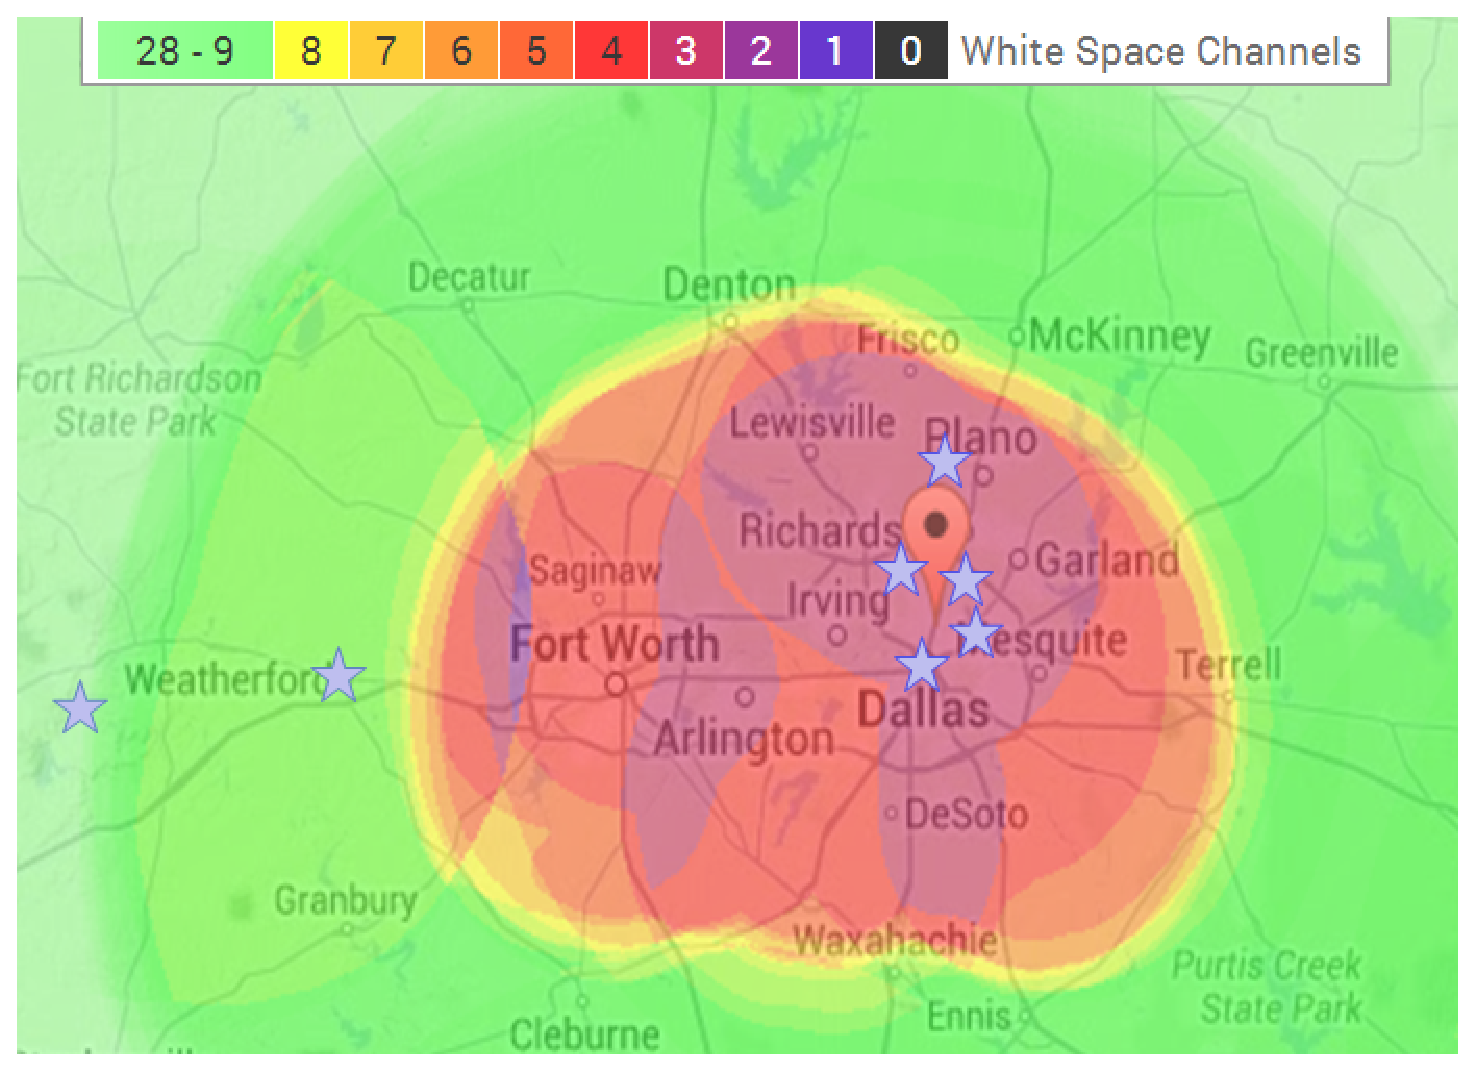
\includegraphics[width=74mm]{figures/drivemap}
\vspace{-0.1in}
\caption{White Space Channels in DFW Metropolitan and Surrounding Areas.}                                                                 
\label{fig:drivemap}
\vspace{-0.1in}
\end{figure}
   
\begin{figure}
%\vspace{-0.0in}
\centering
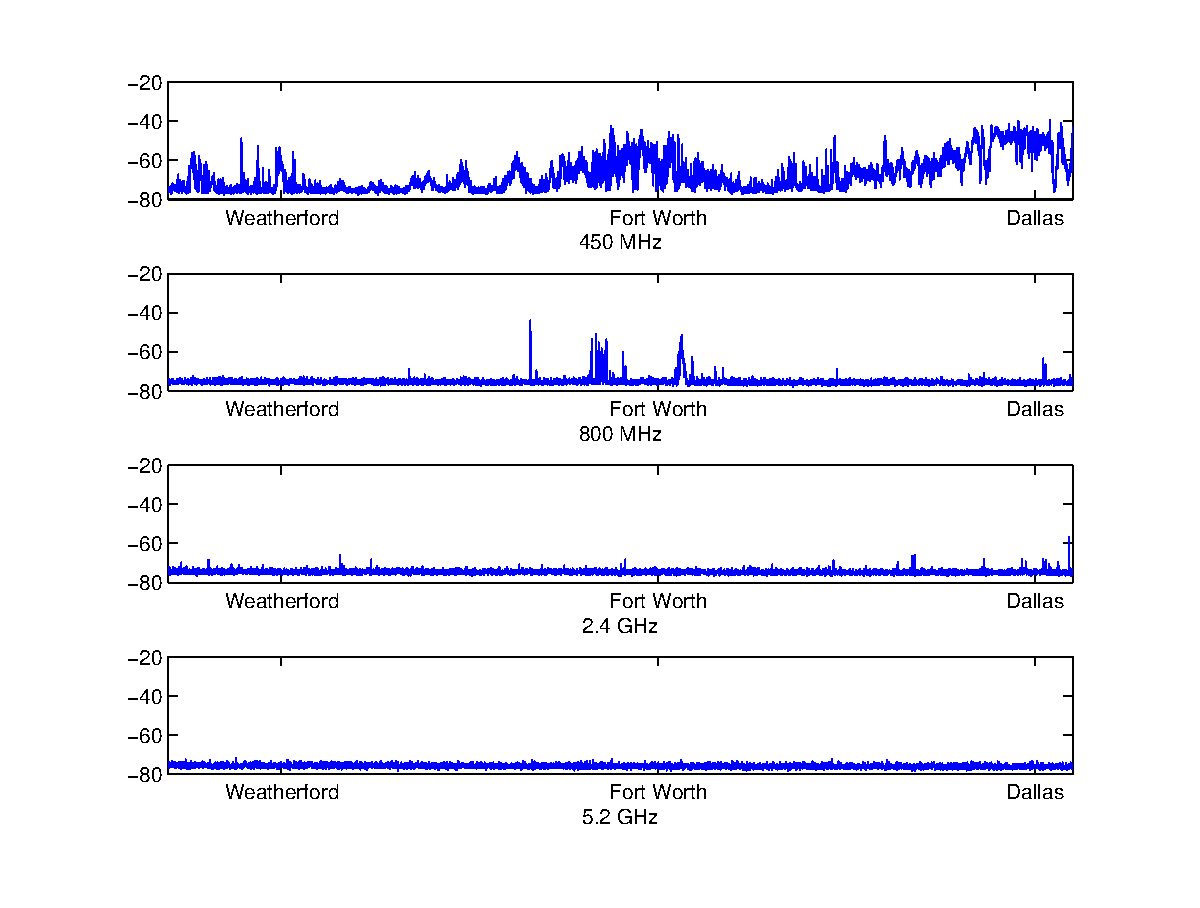
\includegraphics[width=84mm]{figures/drivetest}
\vspace{-0.3in}
\caption{Spectrum Activity in DFW Metropolitan and Surrounding Areas.}                                                                 
\label{fig:drivetest}
\vspace{-0.2in}
\end{figure}




% Here

The activity level calculated with our measurements are shown in Table~\ref{tab:activitymeasurement}. Dallas, the 
city with the greatest population in North Texas, has the highest activity level in most of the measured bands, 
especially at 450 MHz. The Dallas urban measurements are taken from the SMU campus, two neighborhoods, and a 
densely-populated suburb (Plano). Our measurements indicate that 2.4 GHz has a higher activity level in the aforementioned urban areas 
than the measured downtown area. Most schools and their neighborhoods are covered by WiFi, which contributes to the 
high activity level at 2.4 GHz and 5.2 GHz. In Weatherford, all the bands have lower activity levels than in Dallas. 
A peculiarity in the measurements can be seen by the sparse area in Weatherford having more activity than the other 
regions for 450 MHz. This can be explained due to the measurement location being on the East side of Weatherford (closer 
to Fort Worth, which has a population of approximately 750k). Millsap is a typical sparse rural area with approximately 
500 total residents. The activity levels across all the bands are lower than in Dallas and Weatherford. In the 450 MHz 
band, the activity level decreases much faster than in other bands in Dallas and Weatherford. 

\begin{table*}
\centering % centering table 
\begin{tabular}{|l|c|c|c|c|c|c|c|c|c|c|c|} % creating 12 columns 
\hline %\hline % inserting double-line 
Bands     & \multicolumn{3}{c|}{Dallas} & \multicolumn{3}{c|}{Weatherford} & \multicolumn{3}{c|}{Millsap} \\% [0.5ex]
\hline % inserts single-line 
% Entering 1st row 
Area Type & Downtown & Residential & Suburban & Downtown &  Residential & Sparse & Downtown & Residential & Sparse \\ % [0.5ex]
\hline % inserts single-line 
450 MHz &24.37	&25.83  &23.77	&6.05 &12.50  &14.03 & 7.00 & 0.07 & 0.02 \\      
\hline % inserts single-line                                                                                                       
800 MHz &4.40 	&16.49  &4.77	&5.22&5.07 &4.43  & 3.87 & 4.20 & 3.60 \\      
\hline % inserts single-line                                                                                                      
2.4 GHz &15.87 	&34.95  &2.60	&2.03&2.03 &2.77  & 2.07 & 1.60 & 0.80 \\      
\hline % inserts single-line                                                                                                     
5.2 GHz &19.70	&35.46  &1.53	&1.93&1.93 &1.33  & 1.27 & 2.07 & 2.10 \\      
\hline % inserts single-line 
\end{tabular}    
\caption{Activity Level in Multiple Locations} % title name of the table 
\label{tab:activitymeasurement}    
\vspace{-0.3in}
\end{table*}    


% Need a summary
Our measurements verify the channel occupancy variation in the DFW metroplex and quantify the occupancy
through a measurement-based activity level. The results show the spectrum bands have greater occupancy in
densely-populated areas. The measurements 
methods and resulting quantification provides the way to 
understand a typical deployment environment. We apply these 
measurements to our MAPE framework in Section.~\ref{sec:winmee} and BPS algorithms in Section.~\ref{sec:whitemesh} to 
further design access tier network deployments and backhaul tier multiband channel assignment, respectively.

\section{Access Network Deployment Algorithm and Evaluation}
\label{sec:winmee}

In this section, we study the access tier network deployment and propose our measurement-driven MAPE framework with the dynamics 
of WiFi and white space bands. We further apply our MAPE framework with the measurements shown in Section~\ref{sec:measurements}
to investigate the the access tier gain of WhiteMesh in reducing the number of access point in the Dallas-Fort Worth metroplex.

\subsection{Access Network Model and MAPE} 
\label{subsec:winmeemodel}


% Discuss the white space band in access and backhaul
% Traffic demand calculation
Access tiers must satisfy both the coverage and capacity constraints to provide service for users.
The coverage constraint could be calculated according to the propagation model of Eq.~\ref{eq:friis}. 
Generally, a coverage of $95\%$ of 
access tier is acceptable for wireless access networks~\cite{robinson2010deploying}. We represent the capacity 
constraint according to the demand of a service area, which could be calculated as the 
summation of individual demands all over the service area $D_a=\sum\limits_{p\in P} D_p$. Since household demand 
for the Internet has been previously characterized~\cite{rosston2011household}, $D_a$ could represent the 
population distribution $f$ and service area $k$ as $D_a=\sum\limits_{f \in F,k \in K}\bar{D_p}*f*k$. The capacity 
constraint could be represented with an access point set $M$ according to:
\begin{equation}
\label{eq:nlbound}
\sum_{m \in M}\delta_r^m \ge \sum_{f \in F,k \in K}\bar{D_p}*f*k
\end{equation}


% Discuss the application of activity level
Through the measured activity level, the achieved channel capacity could be calculated through the
free time according to:
\begin{equation}
\label{eq:intercap}
\delta_r=\delta*(1-\bar{A})
\end{equation}
Here, the capacity of a clean channel is denoted by $\delta$ under the protocol model. 
With the achieved channel capacity, we could further estimate the capacity of an access point in the access 
tier and link capacity in the backhaul tier.


In a joint white space and WiFi scenario, the activity level varies according to various interfering sources 
and the propagation characteristics induced by the environmental characteristics of the service area. A 
simple method with the least number of access points to cover an area is to use multiple orthogonal 
lower-frequency channels. However, the FCC limits white space band availability for data networks in most 
metropolitan areas in the United States~\cite{googledatabase}. Moreover, the number of channels in each band 
is limited. Too many lower-frequency channels will cause high levels of intra-network interference, 
which will be discussed in the next backhaul tier section. We assume that the cost of the network is proportional to the 
number of access points required for a given user demand (i.e., due to the cost of hardware and installation). 
Therefore, given a geographical region for a new network deployment, we build a measurement-driven framework 
called Multiband Access Point Estimation (MAPE) to compute the required number of access points.


\begin{algorithm}[t]
\small
\caption{Multiband Access Point Estimation (MAPE)}
\label{algorithm:mape}
\begin{algorithmic}[1]
\REQUIRE  ~~\\
$A$: Measured Activity Level \\
$F$: Population Distribution\\
$C$: Clean Channel Capacity\\
$n$: Path Loss Exponent \\
$B$: Available Frequency Bands\\
$M$: Area to be Covered
\STATE Split $M$ in to different type, calculate the traffic demand density $f$
\STATE Calculate in-field channel capacity $\delta_r$ as $\delta(1-A)$
\STATE Get the propagation coverage area radius $R_p$ from the Friis model based on $n,B,F$
\STATE Calculate the QoS coverage radius $R_{QoS}$ of a multiband access point that satisfies the demands of the area
\STATE The coverage radius of a multiband access point is $min\{R_p,R_{QoS}\}$
\STATE Apply a regular-hexagonal deployment to get the number of access points for serving given area $M$
\ENSURE ~~\\
The number of access points\\
\end{algorithmic}
\end{algorithm}

In the spatial domain, the advantage of higher-frequency channels is the spatial reuse, while the lower-frequency 
channels provide greater levels of coverage. Generally, higher frequencies are more appropriate for populated 
areas, and lower frequencies are more appropriate for sparse areas. The temporal variation of spectrum utilization 
differs across bands. For an Internet service provider, the service quality which maps to the capacity constraint 
must be satisfied. Given a metropolitan area, the population distribution can be found according to census data~\cite{uscensus}. 
Then, we can estimate the capacity demand of each type of area with the assumption that users 
will exhibit average demand. According to the population distribution, we split the area into different types,
which compose the spatial input. Then, we use the measured activity level as the temporal input. We have an average 
channel capacity of each band according to the activity level. With the received signal strength threshold, the 
Quality-of-Service-constrained coverage area of different types per channel, and the spatial reuse distance can be 
directly computed. Then, the maximum area an access point could cover can be calculated as the minimal area of the 
QoS-based coverage area and propagation coverage. Then, the transmission power is adjusted to fulfill the coverage 
restriction subject to the FCC regulations for maximum-allowable transmit power. A regular-hexagonal deployment 
process is employed to place the access points. 

\subsection{Results and Analysis}
\label{subsec:winmeeresult}

We use the measurement-based activity levels shown in Table~\ref{tab:activitymeasurement} as an input to 
Alg.~\ref{algorithm:mape}. We specifically use the Millsap sparse area, Millsap downtown, Weatherford residential, 
Dallas residential, and Dallas downtown measurements as inputs of activity level for a given population density. We then 
calculate the number of access points for covering a 13 km $\times$ 13 km area, varying the population density. The 
output is shown in Fig.~\ref{fig:redensity}. 

   \begin{figure}
   %\vspace{-0.0in}
   \centering
   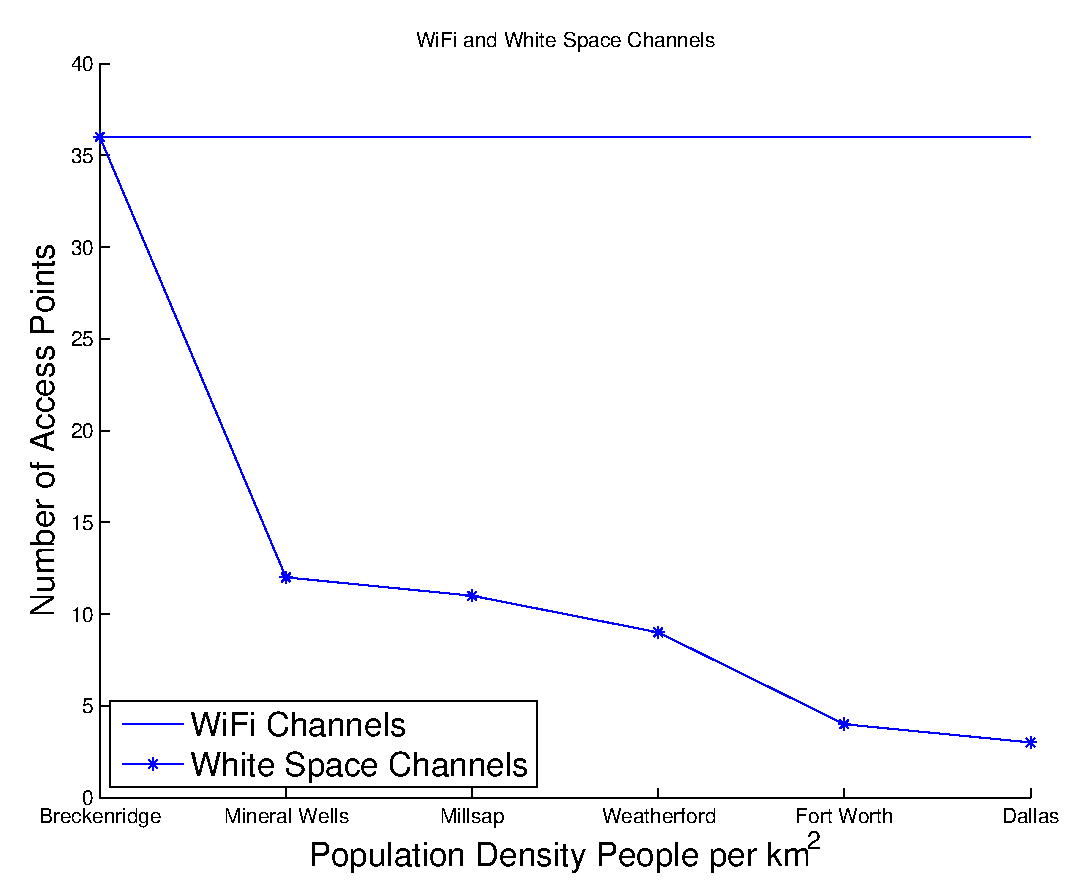
\includegraphics[width=84mm]{figures/redensity}
   \vspace{-0.1in}
   \caption{Number of Access Points Needed for a 13 km x13 km Area.}
   \label{fig:redensity}
   \vspace{-0.3in}
   \end{figure}

% Experiment Results & expect results
In the calculation, we set the demand requested per user to be 2 Mbps with the population density of 20, 50, 100, 1000, 
and 2000 users per square kilometer. We assume 30\% of the residents will use this service (i.e., the take rate is 
30), the maximum transmit power is 30 dBm, with a path loss exponent of $3.5$~\cite{meikle2012global}. From Eq.~\ref{eq:friis}, 
we see that the propagation range is proportional to the wavelength with 450 MHz having a propagation 
range of $11.6$ times that of 5.2 GHz. We adopt an 802.11n maximum data rate of 600 Mbps. For the WiFi+White Space 
scenario, we use 3 channels in each of the 450 MHz, 2.4 GHz and 5.2 GHz bands. For the WiFi Only scenario, we assume 
6 channel in the 2.4-GHz band, and 3 channels in the 5.2-GHz band since 2.4 GHz has a greater propagation range than 5.2 GHz. 
Each of these scenarios have the same channels in total (9). As shown in Fig.~\ref{fig:redensity}, with the same number 
of channels, the WiFi+White Space scenario reduces the number of access points by $1650\%$ compared to the WiFi Only scenario in the 
20 people per square km scenario, $660\%$ in the 50 people per square km, and $412.5\%$ in the 100 people per square km 
scenario. The large propagation range of the white space bands is approximately 10 times that of the WiFi bands, creating 
an opportunity for greater coverage. However, as the population density increases, due to the capacity constraint of 
servicing users in the area, the lower-frequency white space bands lose their advantage of larger communication range due 
to the reduction in achievable spatial reuse. At the same time, the activities of other signal sources, such as TV stations 
in downtown areas, reduce the capacity of white space bands. As a result, the WiFi+White Space scenario performs worse 
than the WiFi Only scenario. If we were to count the intra-network interference as in the following section, the situation could become 
even worse. Moreover, FCC has stricter policies on white spaces in urban areas. Fewer channels are available in the 
downtown and urban areas, which makes WiFi a better option for these dense areas.

To understand the influence of band combinations on network deployments, we calculate the number of access points in the 
area when selecting 500 people per square km with a downtown Weatherford spectrum utilization and 1500 people per square 
km with a residential Dallas spectrum utilization. We assume the total number of channels is 12. We use the same setup 
as the previous experiment.
 
 \begin{table}[h]
 \centering
 \begin{tabular}{|c|c|c|c|}
 \hline
 \multirow{2}{*}{No. of Bands} & \multirow{2}{*}{Bands Combination} & \multicolumn{2}{c|}{No. of AP} \\
 \cline{3-4}
  &  & 500 & 1500 \\
 & (Hz) & $ppl/km^2$ &  $ppl/km^2$ \\
 \hline
 \multirow{4}{*}{1}    & 450 M  & 12  & 35 \\
 \cline{2-4}
                              & 800 M & 10  &  30 \\
 \cline{2-4}
			      & 2.4 GHz & 33  &  37 \\
 \cline{2-4}
                              & 5.2 G & 193 &  193 \\ 
 \hline
 \multirow{6}{*}{2}   & 450 M,800 M & 11  & 32\\
 \cline{2-4}
                              & 450 M,2.4 G & 23  & 36\\
 \cline{2-4}
			      & 450 M,5.2 G & 23  & 69\\
 \cline{2-4}
			      & 800 M,2.4 G & 20  & 33\\ 
 \cline{2-4}
			      & 800 M,5.2 G & 20  & 59\\ 
 \cline{2-4}
			      & 2.4 G,5.2 G & 33  & 73\\ 
 \hline
 \multirow{4}{*}{3} & 450 M,800 M,2.4 G & 16  & 33\\
 \cline{2-4}
                              & 450 M,800 M,5.2 G & 16  & 48\\
 \cline{2-4}
			      & 450 M,2.4 G,5.2 G & 33  & 53\\
 \cline{2-4}
			      & 800 M,2.4 G,5.2 G & 30 &  49\\ 
 \hline
 4  & 450 M,800 M,2.4 G,5.2 G & 21  & 44 \\
 \hline
 \end{tabular}
 \caption{Channel Combinations for $500$ and $1500$ Population Density Scenarios}
 \label{tab:500comb}
 \vspace{-0.4in}
 \end{table}


In Table~\ref{tab:500comb}, we compare the number of access points with 12 channels through all 
the possible combinations of bands. 
% Single band compare
Since purchasing and deploying access points is the primary cost of a wireless 
infrastructure, to simplify the calculation, we only count the number of access points as 
the network's cost. 
When all the channels are in the same band, as the frequency goes up, more access 
points are needed to serve the area due to the limited propagation range. However,
450 MHz does not outperform 800 MHz with a single band at both the 500 and 1500 people per
square km cases because 450-MHz channels have larger measured activity levels. 
White space band channels outperform WiFi bands by up to 1830\% in the single band case
with 500 people per square km, but with 1,500 people per square km, the cost reduction
decreases to only 543\%.
% Two bands 
We now distribute an equal number of channels to two-band combinations and run the experiments 
with the same population densities and spectrum utilization. The results show that the white space band
combination (450 and 800 MHz) performs better than WiFi only (2.4 and 5.2 GHz) by 200\% and
128\% with the people per square km of 500 and 1,500, respectively. In fact, the white space only
scenario (450 and 800 MHz) has almost the same performance as the scenarios with one white band and
one WiFi band (450 MHz and 2.4 GHz; 800 MHz and 2.4 GHz) with 1,500 people per square km.
However, with 500 people per square km, the white space only scenario is much better than any other two-band combination.
% Three bands
White space channels provide up to 87.5\% cost reduction in three-band combination scenarios with
500 people per square km, and up to 33.3\% with 1,500 people per square km.  With four bands,
the number of access points required does not reduce using white space bands.

From Fig.~\ref{fig:redensity} and Table~\ref{tab:500comb}, we show that as the population
density increases, the reduction in number of access points required to meet the same demand 
diminishes. Note that a more optimal allocation of channels in different bands could offer
further cost reductions. We further show that as population and spectrum utilization increase, 
at some point, the performance of white space only scenario could be the same as a combination of
white space and WiFi bands. 


\section{Backhual Network Channel Assignment}
\label{sec:whitemesh}

% Organization of the Sec
In this section, we formulate the channel assignment problem use WiFi and white space bands in concert 
when deploying wireless backhual networks. We then present our integer linear programming model and 
heuristic algorithm to address the problem. 
 
\subsection{WhiteMesh Backhual Architecture}
\label{subsec:architecture}

% Explain multiband vs multichannel Adding channel occupancy here, and also activity level
Many works which rely on such an assumption have focused on the allocation of multiple WiFi channels 
with multiple radios in multihop wireless networks with channels in one band~\cite{doraghinejad2014channel}.
However, as white space bands come to this problem, the propagation variation has to be considered in 
wireless network deployment. The propagation variation brings both spatial and spectrum variation for 
backhual network design.

In this work, we consider the diverse propagation characteristics for four frequency bands: 450 MHz, 800 
MHz, 2.4 GHz, and 5.8 GHz. We refer to the two former frequency bands as white space (WS) bands, whereas
the two latter frequency bands as WiFi bands. Due to the broadcast nature of the wireless medium, 
greater levels of propagation induce higher levels of interference. Also, the more allowed frequency
channels and low level signal activity of white space bands co-exist in sparse areas. Thus, in 
sparsely-populated rural areas, the lower frequencies of the white space bands might be a more appropriate 
choice for multihop paths to gateways having reduced hop count with more capacity. However, as the population 
and demand scales up (e.g., for urban regions), the reduced spatial reuse and greater levels of interference 
of white space bands might detract from the overall channel assignment strategy. In such urban areas, select 
links of greater distance might be the most appropriate choice for white space bands, especially since the 
number of available channels is often inversely proportional to the population (due to the existence of greater 
TV channels).

\subsection{Model and Problem Formulation}
\label{subsec:problem}

To distinguish the dynamics of white space bands, we employ the activity level based on multiple measurements 
in the target area to represent the achieved channel capacity. Correspondingly, a connectivity graph $C$ is 
formed for each band in $B$ such that $C=(V,L,B)$.  If the received signal for a given band is above an 
interference-range threshold, then contention occurs between nodes. 

We extend the conflict matrix in~\cite{tang2005interference} related to various interference per band according 
to $F=(E_{i,j},I_{Set},B)$, where $E_{i,j}$ represents the link and $I_{Set}$ includes all the links are physically 
inside the interference range $D_r$ when operating on each band $b \in B$.

Therefore, the problem we model is: to choose the connectivity graph $C'$ which maximizes the served traffic flow obey 
the constraints of multiband wireless network (defined below). A key challenge is that selecting the optimal channels from
the set $B$ leads to a conflict graph $F$ which cannot be known {\it a priory}. Previous works have proposed several 
coloring, cluster-independent set, mixed linear integer methodology for a single band $b$
~\cite{peng2012efficient,tang2005interference,doraghinejad2014channel}. 
However, these works do not address a reduction in hop count or an increase in spatial reuse and channel occupancy for 
a set of diverse bands $B$. 

% Metrics
In network application, the bottleneck of mesh network capacity has been shown to be the gateway's wireless 
connections~\cite{robinson2008adding}. The metric we use to evaluate the proposed algorithm is the served traffic flow.
Wireless networks are operated and maintained by vendors, such as AT\&T, T-Mobile, who charge the customers based on their data 
through Internet. In practice, the traffic demand of the user obey Poisson distribution\cite{saaty1961elements}, 
we then generated Poisson distributed numbers to represent clients' traffic demands in our simulation. The served traffic 
flow is correlated to the population of the area since each user has similar traffic demand in long term average. The 
employed performance metric of served traffic flow $X$, is represented the traffic arrived at the gateway nodes, where 
in Eq.~\ref{eq:goodput}:
\begin{equation}
\label{eq:goodput}
X=\sum_{w \in W, v \in V}T(w,v)
\end{equation}
The traffic arrived gateway node $w\in W$ considers all incoming and outgoing wireless traffic from access node $v\in V$ 
as $T$ onto the Internet. Obviously, the served traffic flow is also related to the routing and other factors, we use a 
simple routing method to keep the maximum the traffic arrived at the gateway nodes, the exact calculation of served traffic
flow is described in Section~\ref{subsec:wmanalysis}.

\subsection{Linear Programming Formulation}
\label{subsec:linearopt}

To clarify the problem and approach the optimization solution of the problem, we present a linear programming 
formulation for optimizing channel assignment in multiband scenario. We assume that the set of available mesh nodes 
($V$), gateways ($W$), and available bands ($B$) are pre-known. The communication links and conflict graph are 
given as parameters. The capacity $\delta_b$ is given as the achieved channel capacity from the  activity level 
measurement calculation in~\ref{eq:intercap}. 


% Start from here on Fri, finish in the morning
\noindent
{\bf Sets:}
\begin{tabular}{ll}
$V$ & set of nodes \\
$B$ & set of bands \\
\end{tabular}

\noindent
{\bf Parameters:}\\
\\
%\vspace{0.1in}
%\begin{tabular}{lll}
\begin{tabular}{llp{3.4cm}}
%\hline
$\delta^b$ & $b \in B$ & Available capacity of band $b$ in target area\\
%\begin{tabular}{llp{2.8cm}}
$I_{ij,lm}^b$ & $(i,j,l,m) \in V, b\in B $ & Protocol Interference of link $(i,j)$ on band $b$ brought by link $(l,m)$\\
%\hline
%\end{tabular}\\
%\begin{tabular}{llp{2.8cm}}
$W_i$ & $i \in V\ binary$ & Gateway maker in mesh nodes\\
%\hline
%\end{tabular}\\
%\begin{tabular}{llp{2.8cm}}
$D_{d}$ & $i \in V\ $ & Downlink demand of node i\\
%\hline
%\end{tabular}\\
%\begin{tabular}{llp{2.8cm}}
$D_{u}$ & $i \in V\ $ & Uplink demand of node i\\
%\hline
\end{tabular}

In the variable set, we define a time share represents the percentage of time a single link transmits according 
to~$\alpha_{i,j}^b$ for link $i,j$ between node $i$ and node $j$ in band $b$. There are two terms $uy_{i,j,k}^{b}$
and $dy_{i,j,k}^{b}$ defined as uplink and downlink flows:

\noindent
%\vspace{2pt}
{\bf Variables:}\\
\\
%\vspace{1pt}
\begin{tabular}{llp{3cm}}
$0\le \alpha_{ij}^b \le 1$  & $b\in B, (i,j) \in N$ & 
Time share of link $(i,j)$ on band $b$\\ 
$0\le uy_{i,j,k}^b$ & $(i,j,k) \in V, b \in B$ & 
Uplink flow of node $k$ on link $(i,j)$ at band $b$ \\ 
$0\le dy_{i,j,k}^b$ & $(i,j,k) \in N, b \in B$ & 
Downlink flow of node $k$ on link $(i,j)$ at band $b$ \\ 
\end{tabular}
\vspace{1pt}

% FIXME talk about NT calculation
Our objective is represented for  
maximizing the traffic arrived at gateway ($X$)
described in Eq.~\ref{eq:goodput}.

\noindent
{\bf Objective:}
\begin{align}
& Max \sum_i\sum_j\sum_k\sum_b(uy_{i,j,k}^b+dy_{j,i,k}^b) \;\ When \; w_j=1 
%& Max \sum_i\sum_j\sum_b(\frac{1}{\sum_{l,m}\alpha_{i,j}^b\times I_{ij,lm}})
\end{align}

In the ILP, the connectivity, uplink, and downlink constraints are represented as:  

\noindent
%{\bf Constraints:}
{\bf Connectivity Constraints:}
\begin{align}
\label{opt:1}
& \alpha_{i,j}^b + \alpha_{j,i}^b + \sum_l\sum_m(\alpha_{l,m}^b \cdot I_{ij,lm}^b) \leq \delta^b, i\neq j \\
\label{opt:2}
& \sum_i uy_{i,j,k}^b + \sum_i dy_{i,j,k}^b \leq \delta^b \cdot \alpha_{j,k}^b 
\end{align}
\noindent
{\bf Uplink Constraints:} 
\begin{align}
\label{opt:3}
& \sum_k \sum_b uy_{i,k,i}^b \leq D_{ui}  \; ; w_k=0, i \neq k \\
\label{opt:4}
& uy_{i,j,k}^b \cdot w_k = 0 \\
%\label{opt:5}
%& \sum_i\sum_b uy_{i,j,k}^b - \sum_m\sum_b uy_{j,m,k}^b = 0 \; when \; w_k=0, i\neq k\\
\label{opt:6}
& \sum_{i\leq j}\sum_b uy_{i,j,k}^b = \sum_{m\leq j} \sum_b uy_{j,m,k}^b \; ;w_j = 0\\
\label{opt:7}
& uy_{i,j,i}^b=0 
\end{align}
\noindent
{\bf Downlink Constraints:} 
\begin{align}
{\bf}
\label{opt:8}
& \sum_k \sum_b dy_{i,k,i}^b \leq D_{di} \; \; ; w_k=0 \\
\label{opt:9}
& dy_{i,j,k}^b =0  \; ;w_k=1 \\
%\label{opt:10}
%& \sum_j\sum_b dy_{i,j,k}^b - \sum_m\sum_b dy_{i,k,m}^b \geq , i \neq k \\
\label{opt:11}
& \sum_{i\neq j} \sum_b dy_{i,j,k}^b = \sum_{m \neq j} \sum_b dy_{j,m,k}^b   \; ; w_j=0, i \neq k \\
\label{opt:12}
& dy_{i,i,j}^b=0
\end{align}

In the constraints, (\ref{opt:1}) represents the summation of the incoming and outgoing wireless time 
share and the interfering links' wireless time share, which should all be less than 1. Constraint (\ref{opt:2}) 
represents the incoming and outgoing wireless traffic, which should be less than the link capacity for 
link $i,j$. Uplink constraints (\ref{opt:3}) and (\ref{opt:4}) represent that the summation of any wireless 
flow $i,j$ should be less than the demand of node $k$.  Constraints (\ref{opt:6}) and (\ref{opt:7}) are used 
to restrict the sum of all incoming data flows for a given mesh node $k$ to be equal to the sum of all outgoing 
flows. Downlink constraints (\ref{opt:8}) and (\ref{opt:9}) are similar to (\ref{opt:3}) and (\ref{opt:4}) but 
in the downlink direction.  Similarly, constraints (\ref{opt:11}) and (\ref{opt:12}) are downlink versions of 
(\ref{opt:6}) and (\ref{opt:7}).

Similar linear programs model is to solve channel assignment wireless networks have been proved to be NP-hard
~\cite{yuan2006cross}. Our model jointly considers channel assignment factors and multiband scenario which is more
complex . When the particular configuration is given, we further choose the objectives, parameters, and relax 
constraints to find the approaching solution for the network.  

%\section{Path Analysis with Diverse Propagation}
\label{sec:wmalgorithms}


In this section, we discuss the influence of diverse propagation
characteristics of the wide range of carrier frequencies of
% NEWClaim fix
white space and WiFi bands. We then introduce our measurement 
driven heuristic algorithm for channel assignment in 
WhiteMesh networks.

% PEN part 
\subsection{Path Interference Induced on the Network}
\label{subsec:PEN}

In WhiteMesh networks, multihop paths can be intermixed with WiFi 
for more spacial reuse and white space bands with less hops.  
To deal with the trade-off, we consider
analyze the band choices reduce the number of hops along a path and the 
aggregate level of interference that hop-by-hop path choices have
on the network (i.e., Path Interference induced on the Network).

Mesh nodes closer to the gateway generally achieve
greater levels of throughput at sufficiently high offered loads. 
To combat such starvation effects, we treat each flow with equal priority in the network when
assigning channels. In the worst case, all nodes along a particular path have equal 
time shares for contending links (i.e., intra-path interference).
We start the channel assignment assuming that $h$ mesh nodes are demanding
traffic from each hop of an $h$-hop path to the gateway. If each link along the 
path uses orthogonal channels, then each link could be active simultaneously,
otherwise they will complete with each other. 
We note each node along the path had traffic demand $T_d$, obviously the bottleneck 
link along the path would be the one closest to the gateway, and then next. 
Thus, the total traffic along the path $h \cdot T_d$ must be less than the 
bottleneck link's capacity $\delta$ estimated from the measurements. In such a scenario, the $h$-hop mesh node 
would achieve the minimum served demand, which we define as the network efficiency. 
In general, the active time per link for an $h$-hop mesh node can be represented 
by $1,\frac{h-1}{h},\frac{h-2}{h}\cdots \frac{1}{h}$. The summation of all active 
times for each mesh node along the path is considered the intra-path network cost.

Considering only intra-path interference, using lower carrier frequencies allows a
reduction in hop count and increase in the network efficiency of each mesh node along
the $h$-hop path. However, a lower carrier frequency will induce greater interference
to other paths to the gateway (i.e., inter-path interference). 
Fig.~\ref{fig:interferencerange} depicts such an example where
links in different bands are represented by circles for 450 MHz, rectangles for
2.4 GHz, and triangles for the nodes which can choose between the two.
Nodes $A$ and $C$ could be connected through two 2.4-GHz links or a single 450-MHz link.
With 2.4 GHz, the interfering distance will be less than using 450 MHz. For example, only 
link $D,E$ will suffer from interference, whereas $H,I$ would not. However, with 450 MHz,
link $A,C$ would interfere with links $F,G$, $M,L$, and $K,J$. At each time unit, the number of
links interfering with the active links along a path would be the inter-path network cost.

When an $h$-hop flow is transmitted to a destination node, it prevents 
activity on a number of links in the same frequency via the protocol model. 
The active time on a single link can be noted as 
$\frac{T}{\gamma_h}$. 
An interfering link from the conflict matrix $F$ counts as $I_h$ per unit time
and contributes to the network cost in terms of:
$\frac{hT}{\gamma_1}\cdot I_1 + \frac{(h-1)T}{\gamma_2}\cdot I_2 \cdots \frac{T}{\gamma_h}\cdot I_h$.
Then, the traffic transmitted in a unit of network cost for the $h$-hop node is:
\begin{equation}
\label{eq:originpen}
E_{\eta}=\frac{T}{\sum_{i \in h}\frac{(h-i+1)\cdot T}{\gamma_i}\cdot I_i }
\end{equation}
Using network efficiency, the equation simplifies to:
\begin{equation}
\label{eq:pen}
E_{\eta}=\frac{\gamma}{\sum_{i \in h} (h-i+1)\cdot I_i}
\end{equation}

The network efficiency is the amount of traffic that could be 
offered on a path per unit time. With multiple channels from the same band,
$I_i$ will not change due to the common communication range. With multiple
bands, $I_i$ depends on the band choice due to the communication range diversity.  
This network efficiency jointly considers hop count and interference. We define
the Path Interference induced on the Network (PIN) as the denominator of Eq.~\ref{eq:pen},
which represents the sum of all interfering links in the network by a given path. 
PIN is used to quantify the current state of channel for channel assignment
across WiFi and white space bands.
To determine when the lower carrier frequency will be better than two or more hops at a
higher carrier frequency, we consider the average interference $\bar{I}$ of a given path
at the higher frequency.  The problem could be formulated as:
\begin{equation}
\label{eq:benefit}
\frac{\gamma}{\frac{h(h-1)}{2}\cdot \bar{I}+I_x} \geq \frac{\gamma}{\frac{h(h+1)}{2}\cdot \bar{I}}
\end{equation}

Here, from Eq.~ref{eq:benefit} when $I_x \leq 2\cdot h\bar{I}$, the performance of a lower-frequency link  
is better than two higher-frequency hops for the same destination node. $I_x$ is also a parameter of hop count 
in Eq.~\ref{eq:pen}. When the hop count is lower which closer to the gateway node, the threshold 
would be more strict since the interference would have a greater effect on the performance.




\subsection{Band-based Path Selection (BPS) Algorithm}
\label{subsec:BPS}

\begin{algorithm}[t]
    \small
\caption{Band-based Path Selection (BPS)}
\label{algorithms:bps}
\begin{algorithmic}[1]
\REQUIRE  ~~\\
	$M$: Set of mesh nodes\\
	$G$: Set of gateway nodes\\
	$C$: Communication graph of potential links among all nodes\\
	$I$: Interference matrix of all potential links \\
	$B$: Available frequency bands \\
	$\delta$: Measurements based Channel Capacity
\ENSURE ~~\\    
$CA$: Channel Assignment of the Network\\
\STATE Rank mesh nodes in Set $M$ according to physical distance from gateway nodes $G$
\STATE Initialize $S_{curr}=G$, $N_{srv}=\emptyset$, $N_{unsrv}=M$,$I_{active}=\emptyset$
\WHILE {$N_{srv}=!M$}
\STATE Select node with largest distance to gateway
\STATE Find the adjacency matrix across band combinations $A_c$
\FORALL{$A_{i}\in A_c$}
\STATE Find the shortest path $SP_i$ in mixed adjacency matrix A 
\FORALL{Link $l \in SP_i$, ordered from gateway to mesh node}
\STATE Find the least interfering path with measured $\delta \times E_n$
\STATE If equally-interfering links, choose higher frequency
\STATE Calculate the path interference of $SP_i$
\ENDFOR
\STATE Store the shortest path $SP_i$ as $SP$
\ENDFOR
\STATE Assign the path in the network\\
		\STATE Update $N_{srv},N_{unsrv}$
		\STATE Update $I_{active}$ from $I$
\ENDWHILE 

Output $CA$ as the locally-optimal solution\\
\end{algorithmic}
\end{algorithm}

We design a Band-based Path Selection (BPS) algorithm
(described in Alg.~\ref{algorithms:bps}) which first chooses the 
mesh node that has the largest physical distance from the gateway 
nodes to reduce the whole time cost of the network. When a path is constructed for
the mesh node with the greatest distance, all subsequent mesh nodes along
the path are also connected to the gateway. The intuition behind the
BPS algorithm is to improve the worst mesh node performance in a path.
In large-scale mesh networks, it is impractical to traverse all the paths with
different combination of bands from a mesh node to any gateway node since 
it is a NP-hard problem. However,
based on the discussion in Section~\ref{subsec:PEN}, if two paths have the same
number of used bands along those paths, then the path with the least hops
is likely to have the greatest performance and is chosen.  Similarly, if
two path have the same path interference, we choose the path which has
higher-frequency links for spatial reuse. Thus, the next step of the
algorithm is to find the shortest path across band combinations.

To run the algorithm, compared to the number of mesh nodes, the amount of channels $N_B$ in
different bands is small. The time complexity of calculating the combination
is $O(2^{N_B})$. Finding the shortest path in Dijkstra algorithm will
cost $O(N_E^2)$ according to~\cite{golden1976shortest}, where $N_E$ is the set of possible links in the
network, and as a result, the total complexity would be $O(N_E^2\cdot 2^{N_B})$.
The algorithm would then calculate the PIN of the candidate path and select the path
with the least interference channel induced on the network for the source mesh node.
After a path is assigned, the algorithm updates the network's channel assignment
with served nodes, activated links, and radio information. Then,
we iteratively assign channels for all the mesh nodes in the
network.

If all the nodes are connected to gateway nodes ($N_E={n \choose 2}$ which is $O(N_V^2)$), 
then the complexity of assigning a channel for a mesh node is $O(N_E^2\cdot2^{N_B})$. 
Then, the complexity of assigning a mesh node is $O(N_V^4\cdot2^{N_B})$.
To assign {\it all} the nodes in the network, the complexity would 
be $O(N_V^5\cdot2^{N_B})$. The complexity is polynomial time of
the number of traffic demands points (client group) for a wireless
network assignment.



\subsection{Path Analysis with Diverse Propagation}
\label{subsec:wmalgorithms}


We discuss the influence of diverse propagation characteristics of the wide range of carrier frequencies of
white space and WiFi bands in wireless networks. We then introduce our measurement driven heuristic algorithm 
for channel assignment in WhiteMesh networks.

% PEN part 
%\subsection{Path Interference Induced on the Network}
\label{subsec:PEN}

In WhiteMesh networks, multihop paths can be intermixed with WiFi 
for more spacial reuse and white space bands with less hops.  
To deal with the trade-off, we consider
analyze the band choices reduce the number of hops along a path and the 
aggregate level of interference that hop-by-hop path choices have
on the network (i.e., Path Interference induced on the Network).

Mesh nodes closer to the gateway generally achieve
greater levels of throughput at sufficiently high offered loads. 
To combat such starvation effects, we treat each flow with equal priority in the network when
assigning channels. In the worst case, all nodes along a particular path have equal 
time shares for contending links (i.e., intra-path interference).
We start the channel assignment assuming that $h$ mesh nodes are demanding
traffic from each hop of an $h$-hop path to the gateway. If each link along the 
path uses orthogonal channels, then each link could be active simultaneously,
otherwise they will complete with each other. 
We note each node along the path had traffic demand $T_d$, obviously the bottleneck 
link along the path would be the one closest to the gateway, and then next. 
Thus, the total traffic along the path $h \cdot T_d$ must be less than the 
bottleneck link's capacity $\delta$ estimated from the measurements. In such a scenario, the $h$-hop mesh node 
would achieve the minimum served demand, which we define as the network efficiency. 
In general, the active time per link for an $h$-hop mesh node can be represented 
by $1,\frac{h-1}{h},\frac{h-2}{h}\cdots \frac{1}{h}$. The summation of all active 
times for each mesh node along the path is considered the intra-path network cost.

Considering only intra-path interference, using lower carrier frequencies allows a
reduction in hop count and increase in the network efficiency of each mesh node along
the $h$-hop path. However, a lower carrier frequency will induce greater interference
to other paths to the gateway (i.e., inter-path interference). 
Fig.~\ref{fig:interferencerange} depicts such an example where
links in different bands are represented by circles for 450 MHz, rectangles for
2.4 GHz, and triangles for the nodes which can choose between the two.
Nodes $A$ and $C$ could be connected through two 2.4-GHz links or a single 450-MHz link.
With 2.4 GHz, the interfering distance will be less than using 450 MHz. For example, only 
link $D,E$ will suffer from interference, whereas $H,I$ would not. However, with 450 MHz,
link $A,C$ would interfere with links $F,G$, $M,L$, and $K,J$. At each time unit, the number of
links interfering with the active links along a path would be the inter-path network cost.

When an $h$-hop flow is transmitted to a destination node, it prevents 
activity on a number of links in the same frequency via the protocol model. 
The active time on a single link can be noted as 
$\frac{T}{\gamma_h}$. 
An interfering link from the conflict matrix $F$ counts as $I_h$ per unit time
and contributes to the network cost in terms of:
$\frac{hT}{\gamma_1}\cdot I_1 + \frac{(h-1)T}{\gamma_2}\cdot I_2 \cdots \frac{T}{\gamma_h}\cdot I_h$.
Then, the traffic transmitted in a unit of network cost for the $h$-hop node is:
\begin{equation}
\label{eq:originpen}
E_{\eta}=\frac{T}{\sum_{i \in h}\frac{(h-i+1)\cdot T}{\gamma_i}\cdot I_i }
\end{equation}
Using network efficiency, the equation simplifies to:
\begin{equation}
\label{eq:pen}
E_{\eta}=\frac{\gamma}{\sum_{i \in h} (h-i+1)\cdot I_i}
\end{equation}

The network efficiency is the amount of traffic that could be 
offered on a path per unit time. With multiple channels from the same band,
$I_i$ will not change due to the common communication range. With multiple
bands, $I_i$ depends on the band choice due to the communication range diversity.  
This network efficiency jointly considers hop count and interference. We define
the Path Interference induced on the Network (PIN) as the denominator of Eq.~\ref{eq:pen},
which represents the sum of all interfering links in the network by a given path. 
PIN is used to quantify the current state of channel for channel assignment
across WiFi and white space bands.
To determine when the lower carrier frequency will be better than two or more hops at a
higher carrier frequency, we consider the average interference $\bar{I}$ of a given path
at the higher frequency.  The problem could be formulated as:
\begin{equation}
\label{eq:benefit}
\frac{\gamma}{\frac{h(h-1)}{2}\cdot \bar{I}+I_x} \geq \frac{\gamma}{\frac{h(h+1)}{2}\cdot \bar{I}}
\end{equation}

Here, from Eq.~ref{eq:benefit} when $I_x \leq 2\cdot h\bar{I}$, the performance of a lower-frequency link  
is better than two higher-frequency hops for the same destination node. $I_x$ is also a parameter of hop count 
in Eq.~\ref{eq:pen}. When the hop count is lower which closer to the gateway node, the threshold 
would be more strict since the interference would have a greater effect on the performance.



\subsection{Path Interference Induced on the Network}
\label{subsec:PEN}

In WhiteMesh networks, multihop paths can be intermixed with WiFi for more spacial reuse and white space bands 
with less hops. To deal with the trade-off, we consider analyze the band choices reduce the number of hops along 
a path and the aggregate level of interference that hop-by-hop path choices have on the network (i.e., Path 
Interference induced on the Network).

Mesh nodes closer to the gateway generally achieve greater levels of throughput at sufficiently high offered loads. 
To combat such starvation effects, we treat each flow with equal priority in the network when assigning channels. 
In the worst case, all nodes along a particular path have equal time shares for contending links (i.e., intra-path 
interference). We start the channel assignment assuming that $h$ mesh nodes are demanding traffic from each hop of 
an $h$-hop path to the gateway. If each link along the path uses orthogonal channels, then each link could be active 
simultaneously, otherwise they will complete with each other. We note each node along the path had traffic demand 
$T_d$, obviously the bottleneck link along the path would be the one closest to the gateway, and then next. 
Thus, the total traffic along the path $h \cdot T_d$ must be less than the bottleneck link's capacity $\delta$ 
estimated from the measurements. In such a scenario, the $h$-hop mesh node would achieve the minimum served demand, 
which we define as the network efficiency. In general, the active time per link for an $h$-hop mesh node can be represented 
by $1,\frac{h-1}{h},\frac{h-2}{h}\cdots \frac{1}{h}$. The summation of all active times for each mesh node along the 
path is considered the intra-path network cost.

Considering only intra-path interference, using lower carrier frequencies allows a reduction in hop count and increase 
in the network efficiency of each mesh node along the $h$-hop path. However, a lower carrier frequency will induce 
greater interference to other paths to the gateway (i.e., inter-path interference). 
When an $h$-hop flow is transmitted to a destination node, it prevents 
activity on a number of links in the same frequency via the protocol model. 
The active time on a single link can be noted as 
$\frac{T}{\gamma_h}$. 
An interfering link from the conflict matrix $F$ counts as $I_h$ per unit time
and contributes to the network cost in terms of:
$\frac{hT}{\gamma_1}\cdot I_1 + \frac{(h-1)T}{\gamma_2}\cdot I_2 \cdots \frac{T}{\gamma_h}\cdot I_h$.
Then, the traffic transmitted in a unit of network cost for the $h$-hop node is:
\begin{equation}
\label{eq:originpen}
E_{\eta}=\frac{T}{\sum_{i \in h}\frac{(h-i+1)\cdot T}{\gamma_i}\cdot I_i }
\end{equation}
Using network efficiency, the equation simplifies to:
\begin{equation}
\label{eq:pen}
E_{\eta}=\frac{\gamma}{\sum_{i \in h} (h-i+1)\cdot I_i}
\end{equation}

The network efficiency is the amount of traffic that could be 
offered on a path per unit time. With multiple channels from the same band,
$I_i$ will not change due to the common communication range. With multiple
bands, $I_i$ depends on the band choice due to the communication range diversity.  
This network efficiency jointly considers hop count and interference. We define
the Path Interference induced on the Network (PIN) as the denominator of Eq.~\ref{eq:pen},
which represents the sum of all interfering links in the network by a given path. 
PIN is used to quantify the current state of channel for channel assignment
across WiFi and white space bands.
To determine when the lower carrier frequency will be better than two or more hops at a
higher carrier frequency, we consider the average interference $\bar{I}$ of a given path
at the higher frequency.  The problem could be formulated as:
\begin{equation}
\label{eq:benefit}
\frac{\gamma}{\frac{h(h-1)}{2}\cdot \bar{I}+I_x} \geq \frac{\gamma}{\frac{h(h+1)}{2}\cdot \bar{I}}
\end{equation}

Here, from Eq.~ref{eq:benefit} when $I_x \leq 2\cdot h\bar{I}$, the performance of a lower-frequency link  
is better than two higher-frequency hops for the same destination node. $I_x$ is also a parameter of hop count 
in Eq.~\ref{eq:pen}. When the hop count is lower which closer to the gateway node, the threshold 
would be more strict since the interference would have a greater effect on the performance.






\subsection{Band-based Path Selection (BPS) Algorithm}
\label{subsec:BPS}

\begin{algorithm}[t]
    \small
\caption{Band-based Path Selection (BPS)}
\label{algorithms:bps}
\begin{algorithmic}[1]
\REQUIRE  ~~\\
	$M$: Set of mesh nodes\\
	$G$: Set of gateway nodes\\
	$C$: Communication graph of potential links among all nodes\\
	$I$: Interference matrix of all potential links \\
	$B$: Available frequency bands \\
	$\delta$: Measurements based Channel Capacity
\ENSURE ~~\\    
$CA$: Channel Assignment of the Network\\
\STATE Rank mesh nodes in Set $M$ according to physical distance from gateway nodes $G$
\STATE Initialize $S_{curr}=G$, $N_{srv}=\emptyset$, $N_{unsrv}=M$,$I_{active}=\emptyset$
\WHILE {$N_{srv}=!M$}
\STATE Select node with largest distance to gateway
\STATE Find the adjacency matrix across band combinations $A_c$
\FORALL{$A_{i}\in A_c$}
\STATE Find the shortest path $SP_i$ in mixed adjacency matrix A 
\FORALL{Link $l \in SP_i$, ordered from gateway to mesh node}
\STATE Find the least interfering path with measured $\delta \times E_n$
\STATE If equally-interfering links, choose higher frequency
\STATE Calculate the path interference of $SP_i$
\ENDFOR
\STATE Store the shortest path $SP_i$ as $SP$
\ENDFOR
\STATE Assign the path in the network\\
		\STATE Update $N_{srv},N_{unsrv}$
		\STATE Update $I_{active}$ from $I$
\ENDWHILE 

Output $CA$ as the locally-optimal solution\\
\end{algorithmic}
\end{algorithm}

We design a Band-based Path Selection (BPS) algorithm (described in Alg.~\ref{algorithms:bps}) which 
first chooses the mesh node that has the largest physical distance from the gateway nodes to 
reduce the whole time cost of the network. When a path is constructed for the mesh node with 
the greatest distance, all subsequent mesh nodes along the path are also connected to the gateway. 
The intuition behind the BPS algorithm is to improve the worst mesh node performance in a path.
In large-scale mesh networks, it is impractical to traverse all the paths with different combination 
of bands from a mesh node to any gateway node since it is a NP-hard problem. However, based on the 
discussion in Section~\ref{subsec:PEN}, if two paths have the same number of used bands along those 
paths, then the path with the least hops is likely to have the greatest performance and is chosen. 
Similarly, if two path have the same path interference, we choose the path which has higher-frequency 
links for spatial reuse. Thus, the next step of the algorithm is to find the shortest path across 
band combinations.

To run the algorithm, compared to the number of mesh nodes, the amount of channels $N_B$ in
different bands is small. The time complexity of calculating the combination
is $O(2^{N_B})$. Finding the shortest path in Dijkstra algorithm will
cost $O(N_E^2)$ according to~\cite{golden1976shortest}, where $N_E$ is the set of possible links in the
network, and as a result, the total complexity would be $O(N_E^2\cdot 2^{N_B})$.
The algorithm would then calculate the PIN of the candidate path and select the path
with the least interference channel induced on the network for the source mesh node.
After a path is assigned, the algorithm updates the network's channel assignment
with served nodes, activated links, and radio information. Then,
we iteratively assign channels for all the mesh nodes in the
network.

If all the nodes are connected to gateway nodes ($N_E={n \choose 2}$ which is $O(N_V^2)$), 
then the complexity of assigning a channel for a mesh node is $O(N_E^2\cdot2^{N_B})$. 
Then, the complexity of assigning a mesh node is $O(N_V^4\cdot2^{N_B})$.
To assign {\it all} the nodes in the network, the complexity would 
be $O(N_V^5\cdot2^{N_B})$. The complexity is polynomial time of
the number of traffic demands points (client group) for a wireless
network assignment.


\subsection{Evaluation of WhiteMesh Backhual Channel Assignment}
\label{subsec:whitemeshexperimentdesign}

% Adjust the order of the results and explain the result more in detail
We now extensively evaluate our proposed measurement-driven heuristic algorithm against the 
upper bound approaching formed by our integer linear program and versus prior channel assignment 
strategies. We introduce the topologies and metric calculation used in the analysis and present a 
set of results based on the linear program and heuristic algorithm.

\subsection{Experimental Evaluation Setup}
\label{subsec:design}
% Simulation Setup
A key aspect of WhiteMesh networks is the diversity in propagation from the lowest white
space channels (tens to hundreds of MHz) to the highest WiFi channels (multiple GHz). Thus, 
to evaluate the performance of our measurement-driven algorithm, we consider a wide range 
of propagation characteristics from four different frequency bands.  
We have 450 MHz and 800 MHz in white space bands and 2.4 GHz and 5.8 GHz in WiFi bands
in previous measurement work.

% Network Setup
The measurements connect the relation of population distribution, traffic demand,
and available channel capacity in multiple bands. We input the measurements to the ILP and heuristic 
algorithm to calculate the available channel capacity $\delta$ for our algorithm which makes the available 
channel capacity of all the bands more practical. With the same transmission power and antenna gain, the 
highest carrier frequency would have the shortest communication range. Hence, we set a communication-range 
threshold of -100 dBm, and normalize the communication range with the highest frequency of 5.8 GHz. In 
particular, the communication range of 450 MHz, 800 MHz, 2.4 GHz, and 5.8 GHz would be normalized to 12.8, 
6.2, 2.4, and 1, respectively according to Eq.~\ref{eq:friis}. The interference range is computed as twice 
that of the communication range~\cite{raniwala2005architecture}. We deploy static wireless mesh networks of 
$n$ mesh nodes along a regular grid with a normalized distance of 0.8 between rectangular edges. The gateways 
are chosen through a typical cell hexagon deployment method based on 2.4 GHz~\cite{meguerdichian2001exposure}.
Unless otherwise, specified in the analysis, all four bands are used in the WhiteMesh topology studied. For 
practical application scenarios, more channels could be involved in the algorithms.

% Traffic generation
As discussed in~\ref{subsec:problem}, the traffic demand obey Possion distribution. The traffic demand 
aggregated by a mesh node is independent to others. In the simulation, we generate an equal number of 
access points (including both gateway nodes and mesh nodes) Possion random numbers with an expect $\lambda$ 
according to the population distribution for the target area. Then we map the number to the traffic demand 
for each access points in the target area.
% Served traffic flow calculation
The served traffic flow is not only critical for network vendors (e.g., cellular carriers charge fees for 
total bandwidth through towers), but also has been used by researchers to evaluate channel assignment~\cite{avallone2008channel}. 
As mentioned previously, the wireless capacity of gateway nodes has been shown to be the bottleneck in mesh 
networks~\cite{robinson2010deploying}. Moreover, served traffic flow is affected by multiple factors, such 
as mesh node placement, gateway placement, routing, and channel assignment, the latter of which is the focus 
of our analysis and algorithms. For the purposes of our analysis, we specifically calculate the served traffic 
flow introduced in Section~\ref{subsec:problem}. After the channel assignment process, the network is under a 
tree based structure. We start to serve the traffic demand from the gateway nodes. Mesh nodes that have a close 
hop count path to the gateway nodes are the first ones served. Where there are nodes with the same hop count, 
the least interfering mesh nodes are chosen for serving. Then, the demand of multihop mesh nodes are served 
until there is no remaining demand to be satisfied or there is no remaining channel capacity through any path.

In the simulations, we investigate the impacts of network size, bands availability, and 
channel occupancy on wireless white mesh networks. We vary the average population distribution 
and the available channel capacity of the target area according to the measurements, assuming 10\% of 
the residents will use our service. An individual would have a 100 KB/s traffic demand on average. 
Then, we assign the demand to users randomly under the same average value across the area and run 
the analysis of each case 20 times as the simulation configuration. Through the assignment, 
the traffic arrived at gateway nodes and the network throughput are calculated. To approach the 
traffic arrived gateway up-bound, we relax our LP model to keep the link capacity constraints, 
given the demand of the mesh nodes as a parameter to achieve the maximum throughput at the gateways. 
We compare BPS with the 
{\it (i)} Common Channel Assignment (CCA) from~\cite{draves2004routing},
{\it (ii)} Breath First Search Channel Assignment (BFS-CA) from~\cite{tang2005interference}
under the same simulation setup.
In typical CCA~\cite{draves2004routing} algorithm, two nodes will assign a common channel 
for each other when both of them share free radios working in the same channel. 
In BFS-CA~\cite{tang2005interference} algorithm, a node will search all the 
available single-hop connections then choose the one has the largest available capacity 
for a new assignment. These two methods focus on multi-channel assuming the existing 
links are equal when there is no assignment on the channel. In BPS, we both consider and 
leverage propagation differences of diverse bands.
The LP Bound calculation make the mesh nodes activate all possible connection 
the gateways if there exists a path. However, the three heuristic algorithms 
provide assignment each mesh node has connection only to one gateway in the 
network, and this reduce the dynamic changes for the assignment, which could be 
implemented by updating the assignment in a short term through the heuristic algorithms.

\subsection{Experimental Analysis of WhiteMesh Backhaul}
\label{subsec:wmanalysis}

\subsubsection{Network Size \& Bands Effect}

% ILP bound
Typically, clients and mesh nodes have diverse traffic patterns with
the download direction dominating the total traffic demand (e.g., consider
service agreements for cellular data or Internet connectivity). Hence, to
simplify the analysis and scale the LP Bound to larger network sizes, we 
only consider the download traffic while maintaining the simulations.
We then assign distributed download traffic demand randomly per 
mesh node with a maximum offered load to simulate the practical scenario 
as specified in Fig.~\ref{fig:all3figs} and Table~\ref{tab:2channelcombination}. 
We average the results of 20 simulations each of the algorithms for the 
given network configuration and compare the results to analyze multiband 
application in wireless network.

First, we investigate network sizes impacts on wireless white mesh network. 
The number of mesh nodes is varied from $16$ to $64$ in the aforementioned 
regular grid. As the network size grows, so too does the number of gateways
through the hexagon gateway nodes deployment. 
Fig.~\ref{fig:varysize} shows the served traffic flow when the 
population distribution is 500 $ppl/km^2$ for the ILP formulation and 
the heuristic algorithms: 
{\it (i)} Common Channel Assignment (CCA) from~\cite{draves2004routing},
{\it (ii)} Breadth First Search Channel Assignment (BFS-CA) from~\cite{ramachandran2006interference},
{\it (iii)} our algorithm BPS (Section~\ref{subsec:BPS}).


\begin{figure}[t]
\centering
\subfigure[Average Population Distribution = 500 $ppl/km^2$]{
\label{fig:varysize}
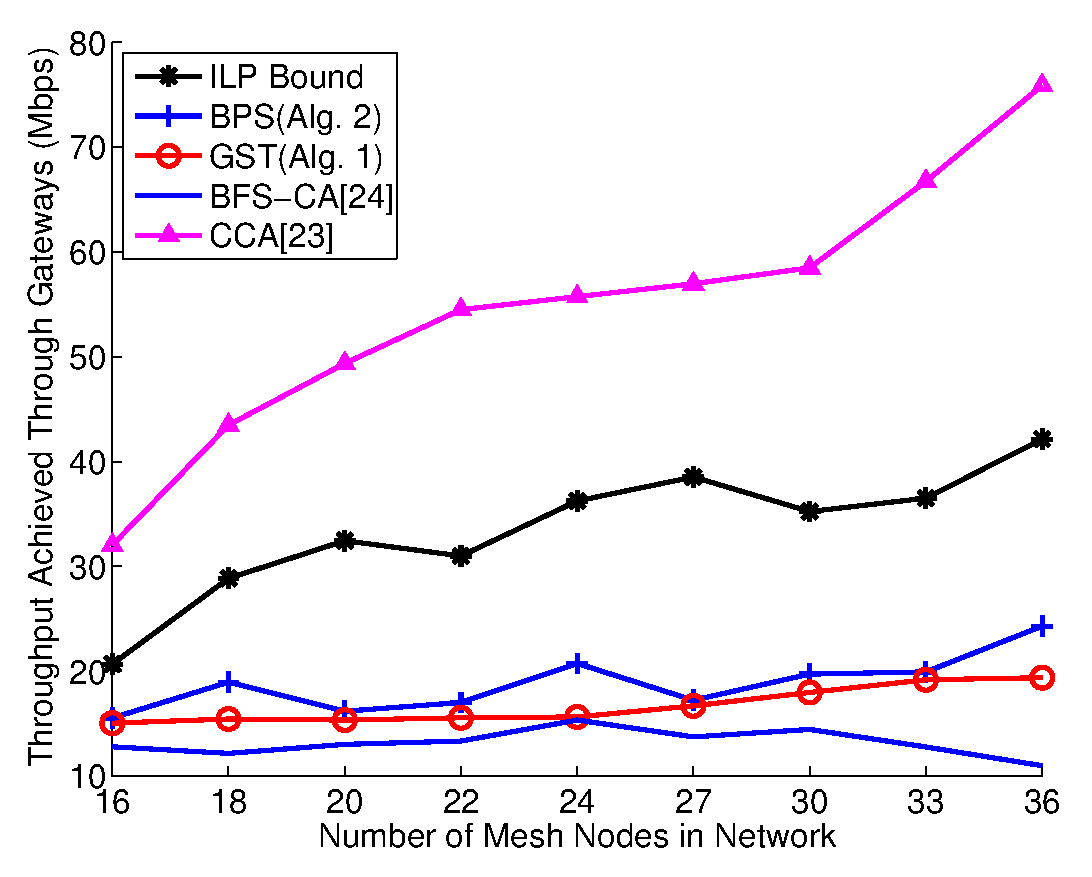
\includegraphics[width=1.6in]{figures/varysize}}
\subfigure[Varying Load, 49-Nodes Regular Grid]{
\label{fig:maxtpt}
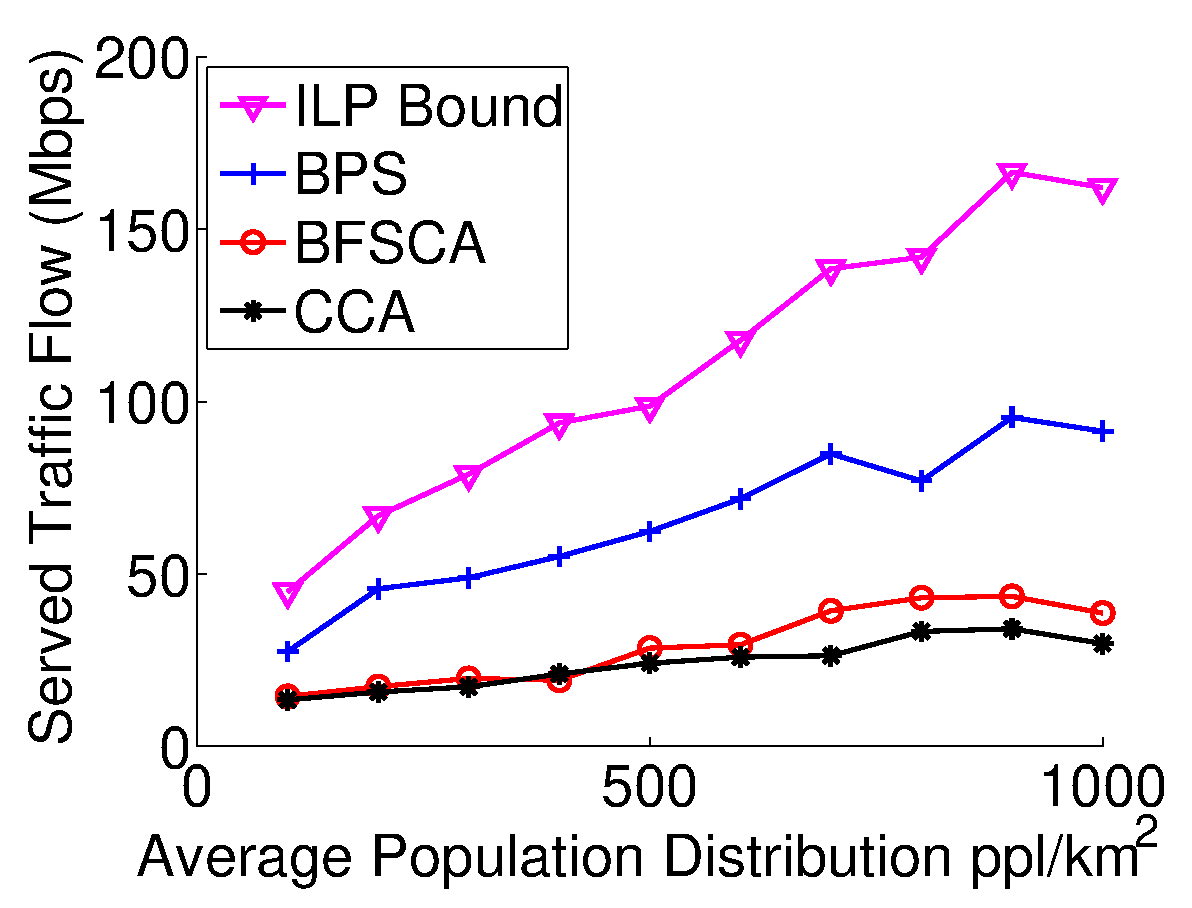
\includegraphics[width=1.6in]{figures/maxtpt.eps}}
\hfill
\caption{Performance in terms of served traffic flow for various offered loads, network sizes, and configurations of WiFi or white space (WS) channels.}
\label{fig:all3figs}
\vspace{-0.1in}
\end{figure}
%\end{figure*}

In Fig.~\ref{fig:varysize}, we observe as the network size increase, the performance
gap among BPS and CCA/BFS-CA goes up. When the network size which represent the size 
of target area, the multiband wireless network has similar communication and interference 
performance with the multi-channel wireless network since all the nodes are located in a 
limited space where could be communicated/interfered by all the bands. As network size 
increase, the connection/interference variation among multiple bands makes the performance 
of multi-channel algorithms stay in low level. The LP Bound shows what could be expected, 
that an increasing number of gateways/mesh nodes produce an increase in total traffic 
arrived gateways. However, we observe that CCA, BFS-CA algorithms are not able to achieve 
such behavior for various reasons. CCA fails to employ the communication range variation 
and find the most efficient hop connections which increase the average hop count. BFS-CA 
optimizes the first connection hop from the gateway, but fails to deal the whole path 
from the gateway to destination node. Conversely, BPS alleviates the strain on these 
first-hop, bottleneck links, achieving average 76\% of the ILP Bound. The gap of BPS 
to the ILP is part from that the BPS only considers static one path to a gateway node for 
each mesh node, whereas the LP allows multiple paths to the gateways. For BPS and other 
heuristic algorithms the dynamic assignment could be implemented through updating the 
assignment in a short term.

\begin{table*}
\centering % centering table 
\begin{tabular}{|c|c|c|c|c|c|c|c|c|c|c|c|} % creating 12 columns 
\hline %\hline % inserting double-line 
%Bands     & \multicolumn{3}{c|}{Dallas} & \multicolumn{3}{c|}{Weatherford} & \multicolumn{3}{c|}{Millsap} \\% [0.5ex]
%\hline % inserts single-line 
% Entering 1st row 
 \multirow{2}{*}{Frequency Bands} & \multicolumn{9}{|c|}{Population Distribution $ppl/km^2$} \\
\cline{2-10}
		& 1500 & 1000 & 500 & 300 &  200 & 150 & 100 & 20 & 10 \\ % [0.5ex]
\hline % inserts single-line 
450 MHz &24.37	&25.83  &23.77	&6.05 &12.50  &14.03 & 7.00 & 0.07 & 0.02 \\      
\hline % inserts single-line                                                                                                       
800 MHz &4.40 	&16.49  &4.77	&5.22&5.07 &4.43  & 3.87 & 4.20 & 3.60 \\      
\hline % inserts single-line                                                                                                      
2.4 GHz &15.87 	&34.95  &2.60	&2.03&2.03 &2.77  & 2.07 & 1.60 & 0.80 \\      
\hline % inserts single-line                                                                                                     
5.2 GHz &19.70	&35.46  &1.53	&1.93&1.93 &1.33  & 1.27 & 2.07 & 2.10 \\      
\hline % inserts single-line 
\end{tabular}    
\caption{Activity Level under Population Distribution} % title name of the table 
\label{tab:activitymeasurement}    
\vspace{-0.3in}
\end{table*}    

% Simulation set up
Next, we consider a different form of scalability in our analysis.  Namely,
we increase the average population distribution from 100 to 1,000 per km$^2$, while
maintaining a 49-node regular grid topology. In the simulation set up, we map the
channel capacity to the closest population measurement results. If there are 
measurements has the same distance to the current set up, the lower population 
measurement will be chosen, for instance, we map $400 ppl/km^2$ to $300 ppl/km^2$ 
measurements as shown in Table.~\ref{tab:activitymeasurement}. In Fig.~\ref{fig:maxtpt},
it shows that as the population distribution increases, the ILP and BPS diverge greatly 
from the remaining algorithms. Similar to Fig.~\ref{fig:varysize}, the wireless channel 
capacity around a gateway is quickly saturated if the algorithm is not focused on 
preserving that resource. Another factor of the performance is the channel capacity, 
as population increase the measured channel capacity vary in different bands.
As the population reaches 1,000, the traffic arrived gateways decrease due to the 
channel capacity and the saturation of wireless channel capacity around the gateway
nodes. BPS has an average performance of 60\% of the ILP Bound, on average. CCA and BFS-CA
fails to serve more traffic demand through the jointly WiFi and white space wireless
network. 

\begin{table*}
\centering % centering table 
\begin{tabular}{|l|c|c|c|c|c|c|c|c|c|c|c|} % creating 12 columns 
\hline %\hline % inserting double-line 
Bands/     & WiFi    & WS      & WS \& & WS \& &  WS \& & WS \& & WS \&      &  WS \&      & Multi-WS \& & Multi-WS \& & Multi-WS \& \\% [0.5ex]
Algorithms & Only    & Only    & WiFi  & WiFi  &  WiFi  & WiFi  & Multi-WiFi &  Multi-WiFi & WiFi        & WiFi        & Multi-WiFi  \\
\hline % inserts single-line 
% Entering 1st row 
WS (MHz)   &                                                        & 450,800 & 450 &  800  &  450   & 800               & 450    & 800      & 450,800     & 450,800     & 450,800     \\
\hline
WiFi (GHz) & 2.4, 5 &                                                             & 2.4 &  2.4  &  5   & 5               & 2.4, 5& 2.4, 5        & 2.4             & 5         & 2.4, 5     \\ % [0.5ex]
\hline
\hline % inserts single-line 
CCA~\cite{draves2004routing}                & 22.4   &  13.4  & 13.2    &12.5    & 16.9       & 23.2   &  24.1  &   30.6&  25.2  &       23.9       &   30.4          \\      
\hline % inserts single-line                                                                                                       
BFS-CA~\cite{ramachandran2006interference}  & 26.3   &  15.8  & 14.9    & 19.4   & 22.7       & 28.4   &  38.9  &   33.7&  30.1  &       27.4       &       36.6      \\      
%\hline % inserts single-line                                                                                                      
%GST (Alg. 1)                                                            & 11.6  &   6.6 & 9.3    &   15.1&   15.8        &  14.4  &   16.6   &    14.1  &   18.8            &  15.0           &    25.1         \\      
\hline % inserts single-line                                                                                                     
BPS (Alg. 1)                                & 41.2   & 34.1   &  38.2  & 40.0    & 35.4       & 42.8   & 58.4   &  64.9 &  54.4  &       51.9       &       63.1      \\      
\hline % inserts single-line 
\end{tabular}    
\caption{Throughput achieved through Gateway nodes (Mbps) for various combinations of WiFi and Average Population Distribution = 500 $ppl/km^2$, Network Size = 49 mesh nodes).} % title name of the table 
% NEWClaim fix
\label{tab:2channelcombination}    
\vspace{-0.4in}
\end{table*}    


WhiteMesh networks could be deployed across a vast array of environments, from
rural to urban areas. Each of these areas will have varying amounts of user
demand traffic in proportion to the population densities.  However, 
since a greater number of TV stations exist in urban areas, the available 
white space bands are often inversely related to the population density due to 
the FCC rules~\cite{fccwhitespace}. Also the available channel capacity is 
related to the existing signal activities in the area. To capture these varying
degrees of demand and white space availability we consider three likely scenarios
and one final scenario for comparison purposes: {\it (i)} two WiFi bands (2.4 and
5.8 GHz) channels with two white space channels (450 and 800 MHz), {\it (ii)} 
three channels in two WiFi bands (2.4 and 5.8 GHz) with one white space channel 
(450 MHz), {\it (iii)} Four channels in two WiFi bands (2.4 and 5.8 GHz) without 
any white space channels, and {\it (iv)} four channels in two white space bands 
(450 and 800 MHz) with no WiFi bands (for comparison).

Table~\ref{tab:2channelcombination} describes the achieved traffic arrived gateways 
for various combinations of WiFi and white space bands with a maximum offered load 
of 5 Mbps from 500 $ppl/km^2$ in a regular 49-node grid. We consider the performance 
of BPS in the four aforementioned scenarios of varying white space availability. A 
regular, 49-nodes grid is again used. In the simulation, we keep 4 channels for each
method, such as in the combination of 2.4 GHz and 5 GHz, we put 2 channels in both 
bands. In the triple bands combinations, we set each band has a channel, and put the 
other channel in the highest frequency band. (In 2.4 GHz, 5GHz, 800 MHz combination, 
we put the extra channel other than the 3 channel each band in 5 GHz). 
% Justification
Immediately, we observe that the WiFi-only scenario has greater traffic arrived 
gateways than the white-space-only scenario. This is due to the lack of spatial 
reuse achieved by white spaces. White space has larger communication to shorten 
the hop counts as well as has larger interference reducing the spatial reuse. 
Another reason is that the available channel capacity of 500 $ppl/km^2$ in white 
space bands are worse than WiFi bands. This two reasons make the white space only 
has worse performance no matter what channel assignment methods are applied.
Interestingly, however, the joint use of both white space and WiFi bands has 
significant gains over the single type of band scenarios with the same number of 
channels (40\% greater than WiFi and 56\% over white space, on average). 

In 500 $ppl/km^2$ scenario, 5 GHz channel is cleaner than 450 MHz which makes 
the combination of 2 channels in 5 GHz, 1 channel in 2.4 GHz and 800 MHz has 
better performance than WiFi(2)+WS(2) in some cases.  Obviously, in Table
~\ref{tab:2channelcombination} that with the same number of available bands (2), 
when the combination has similar propagation characters, such as one in WiFi band, 
one in white space band, the combination has clean channels have better performance. 
With similar channel capacity, lower frequency offers more option for connection 
path could output a better channel assignment. If we have one channel in a white 
space band and one channel in a WiFi band, then we could use the advantage of both 
WiFi for spatial reuse and white spaces to reduce the hop count. 



\subsubsection{Effect of Channel Occupancy}

% FIXME include 3 d figure
In Fig.~\ref{fig:actspac}, we show the impacts of channel occupancy through 
the activity level and spacing variation on wireless white space mesh network. 
The activity level defined in~\ref{eq:intercap} represent the available channel
capacity. The spacing gap is related to the population distribution according to 
the hexagon deployment for access tier network deployment, the more population
distribution, the smaller spacing gap between mesh nodes. In the simulation, we 
assume all the bands have the same activity level and use the 49-nodes regular 
grid with normalized multiple spacing distance gap from 0.2 to 2.1. From the 3-D 
figure, we could see as the activity level increase, the traffic arrived gateways 
decrease due to the deduction of available channel capacity. In the spacing dimension, 
when the nodes have small spacing gap, all the bands could not be applied for 
spacial reuse, the traffic arrived gateways is small. But as the spacing gap 
increase, the spacial reusing is available for high frequency bands, the traffic 
arrived gateways increase. Then, as the spacing gap increase over the high 
frequency communication range, the number of usable channels start to decrease 
according to protocol model, the traffic arrived gateways decrease in the figure.

We further investigate the spacing gap variation under in-field scenario.
The in-field measurement mapping is listed in Table.~\ref{tab:activitymeasurement}. 
We keep the white mesh network as 49-nodes regular grid, assume each mesh 
node has 4 radios in each band. As clarified, a larger spacing gap between mesh 
nodes means less population. We map the largest population distribution in Table
~\ref{tab:activitymeasurement} to represent the spacing as normalized distance 0.2,
and the least population distribution as normalized distance 1.7. 
In a regular grid the spacing distance $D_s$, population distribution $P_d$ and 
mesh node capacity $M_c$ should obey $P_d \cdot \frac{D_s}{2} ^2 \propto M_c$. 
The 9 measured data sets are mapped to generate the matrix sets. Then according 
the data in the matrix we interpolate activity level for each normalized distance 
from 0.2 to 1.7 with gap 0.1. These data sets are put into the heuristic algorithms 
and the results are shown in Fig.~\ref{fig:measurespacing}.

\begin{figure}[t]
\centering
\subfigure[Uniform Activity Level VS. Space Distance]{
\label{fig:actspac}
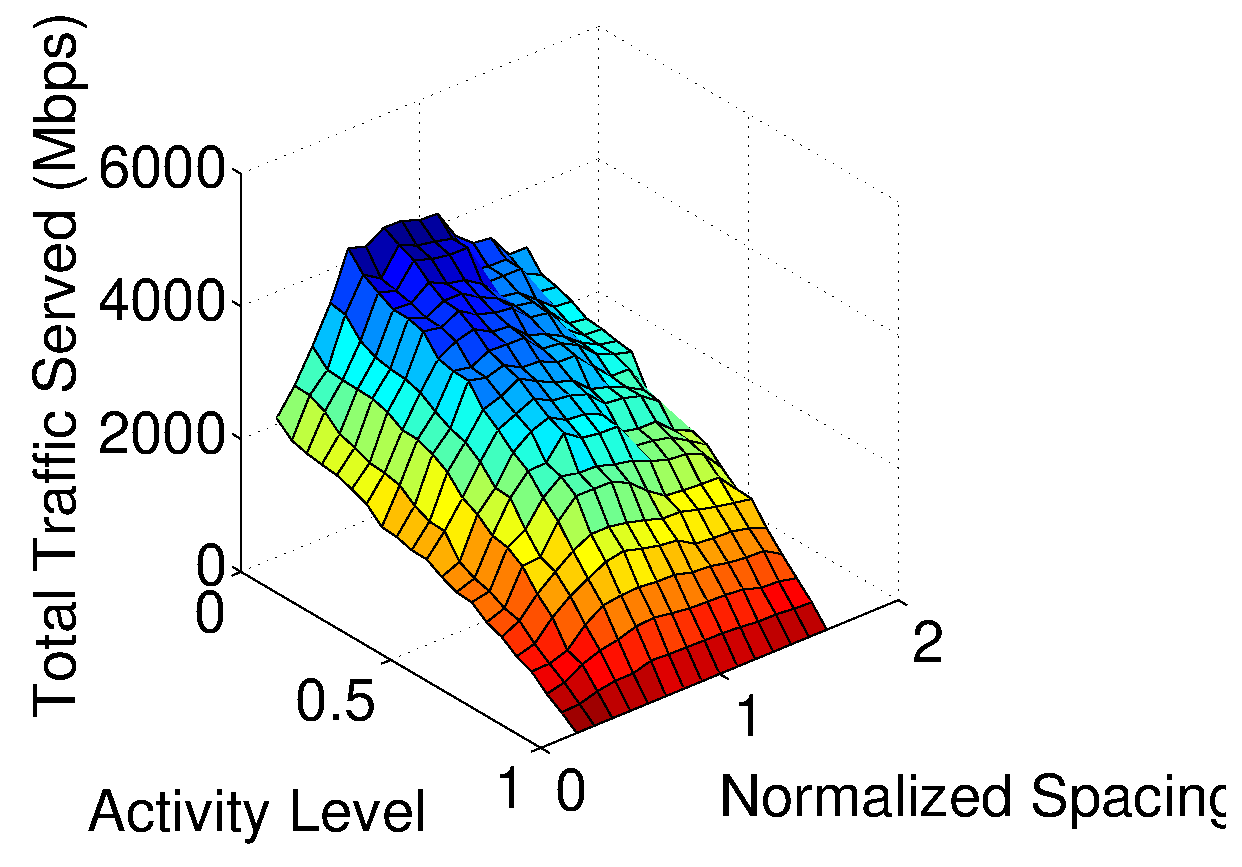
\includegraphics[width=1.6in]{figures/actspac3d}}
\subfigure[Traffic arrived Gateways with Activity Level \& Spacing ]{
\label{fig:measurespacing}
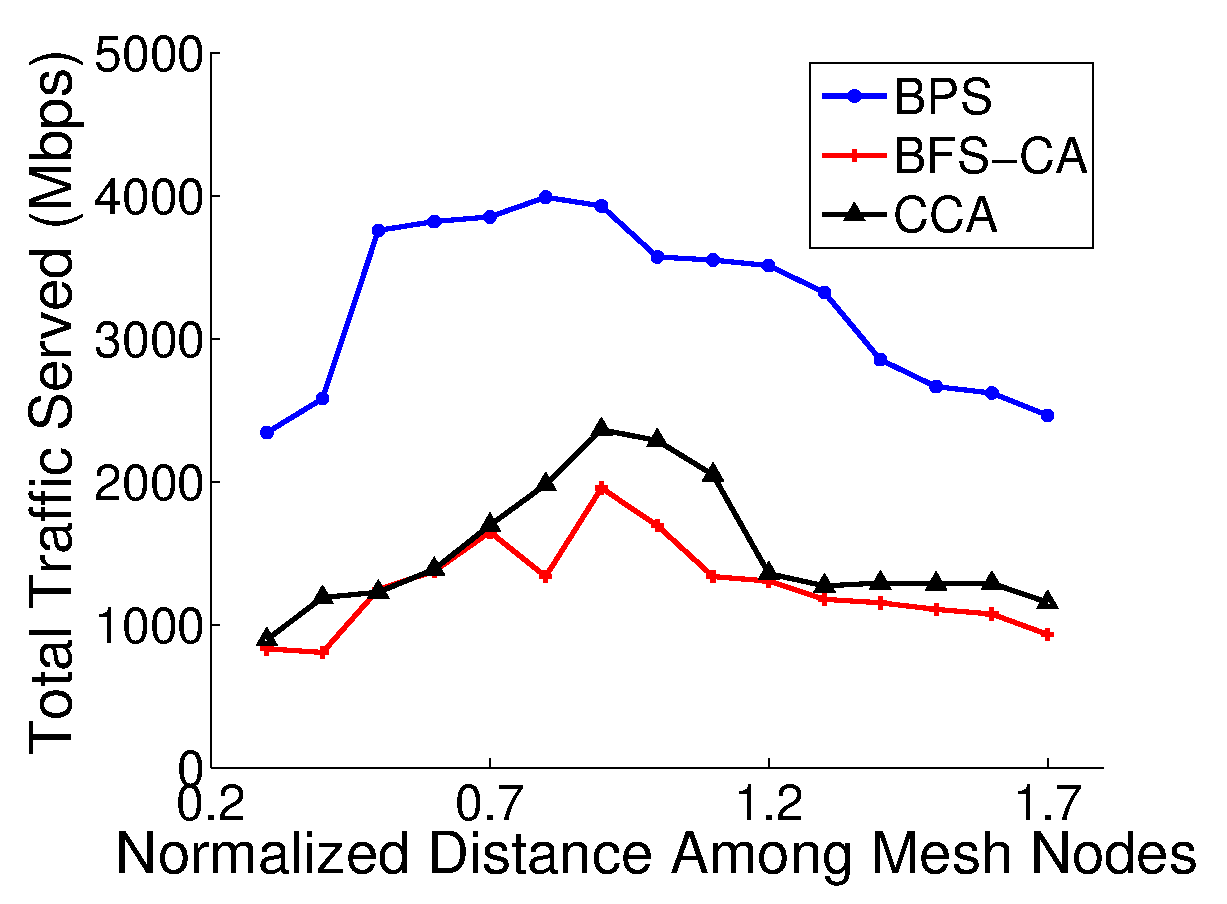
\includegraphics[width=1.6in]{figures/act_spacing}}
\hfill
\caption{}
\label{fig:all3figs}
\vspace{-0.1in}
\end{figure}

In Fig.~\ref{fig:measurespacing}, as the space gap increase, the multiband network 
has better performance through spacial reuse matching the simulation analysis shown 
in Fig.~\ref{fig:actspac}. As the distance increase up to normalized distance 1, one of 
the channel in 5 GHz could not be applied in the network since the distance is larger 
than its communication range under the protocol model, that makes the performance 
decrease quickly. Through this investigation, we can conclude that in sparse area
when the number of mesh nodes is small, lower frequency for the back-hual network 
could have better performance. However, in dense area when the mesh nodes are deployed 
closely, have higher frequency for spacial reuse is better than the low frequency 
white space bands.


Through these analysis, a mixed WiFi and white space wireless network could improve the performance 
in the scenarios as follow: 
{\it (i)} Larger network has more mesh nodes, which 
need more capacity from spacial reuse and flexible path to reduce hop count through
more links. 
{\it (ii)} Rural area whose spacing gap among mesh nodes is larger.
Not only for the number of mesh nodes reducing but also for hop count reducing.
However, as we discussed, the flexible paths and the interference among these
links become more critical at different points in the WhiteMesh topology. 
For the sake of completeness, we need cautious selection of frequency bands
in wireless network deployment.



\section{Related Work}
\label{sec:related}
% Deployment problem 
There are significant challenges in wireless mesh network deployment,
such as user priorities, user behaviors, long term throughput estimation, 
interference and energy efficiency, etc.~\cite{tragos2013spectrum}
Previous works have recognize the impact of interference in wireless mesh network 
deployment is the key issue~\cite{tang2005interference,irwin2013resource,chieochan2013channel}.
To overcome the challenges, previous works have been done to optimize the 
deployment in increasing throughput, minimize resource, reducing interference,
etc~\cite{irwin2013resource,subramanian2008minimum,doraghinejad2014channel}.
Many works have studied the network deployment problem in multihop wireless networks
~\cite{jain2005impact,akyildiz2005wireless,raniwala2004centralized,tragos2013spectrum}.
Both static and dynamic network deployments have been discussed in previous works under
the 802.11 WiFi scenario~\cite{wu2006analysis,ramachandran2006interference,subramanian2008minimum}. 
However, all of the aforementioned works have not considered propagation variation of the 
diverse frequency bands among white space and WiFi, which we show are critical improving 
the performance of mesh networks. Frequency agility in multiband scenario brings more 
achieved channel capacity to wireless network deployment as well as more complexity of 
resolving the interference issues.

% White Space
To be used effectively, white space bands must ensure that available TV bands
exist but no interference exists between microphones and other devices~\cite{bahl2009white}. 
White space bands availability has to be known in prior of network deployment.
TV channels freed by FCC are fairly static in their channel assignment, 
databases have been used to account for white space channel availability 
(e.g., Microsoft's White Space Database~\cite{msdatabase}).
In fact, Google has even visualized the licensed white space channels 
in US cities with an API for research and commercial use~\cite{googledatabase}.
In contrast, we study the performance of mesh networks with a varying number 
of available white space channels at varying population densities, assuming 
such white space databases and mechanisms are in place. As FCC release these 
bands for research, many methods have been proposed to employ these frequency bands.
~\cite{bahl2009white} introduce WiFi like white space link implementation on USRP and 
link protocols. ~\cite{cui2013leveraging} discuss the point to point communication
in multiband scenario. In~\cite{filippini2013new}, white space band application is 
discussed in cognitive radio network for reducing maintenance cost. 
In this work, the objective is maximizing the served traffic flow of clients in the wireless network.






\section{Conclusion}
\label{sec:conclusion}
In this paper, we jointly considered the use of WiFi and white space bands application
for wireless networks deployments. 
Different from prior work, we first proposed a Multiband 
Access Point Estimation (MAPE) framework to estimate the number of access points required in 
a given region for wireless access network and Band-based Path Selection (BPS) algorithm for
backhual network based on in-field measurements for wireless access network. 
We then performed spectrum utilization measurements in the DFW metropolitan and surrounding areas 
to drive these framework and find the influence of white spaces on network costs in these representative areas. 
%
%Further, we investigate different 
%band combinations in two population densities to show that greater access to white space 
%channels have greater total savings of mesh nodes when the total number of channels used 
%in the network is fixed (i.e., given a total number of allowable WiFi and white space channels). 
Through extensive analysis across varying population density and channel combinations across bands, 
we show that white space bands can reduce the number of access points by 1650\%
and 660\% in rural and sparse urban areas versus the same cost savings are not achieved in dense urban 
and downtown type area. As the population and spectrum utilization increase, the cost savings of 
white space bands diminish to the point that WiFi-only channel combinations can be optimal.
The simulation shows that our BPS algorithm can achieve 180\% the served user demand versus previous 
multi-channel, multi-radio solutions in multiband scenarios, since we leverage diverse propagation 
characteristics offered by WiFi and white space bands. Moreover,we quantify the degree to which the joint 
use of these bands can improve the served user demand. Our BPS algorithm shows that WhiteMesh topologies 
can achieve up to 160\% of the served traffic flow of similar WiFi or white-space-only configurations.
% Future work
%In the future, we will consider the heterogeneous access points and traffic demand scenarios
%in wireless network deployments.




\bibliographystyle{IEEEtran}

\bibliography{whitemesh}

\end{document}
%This is never printed
